\documentclass[../thesis.tex]{subfiles}

\begin{document}
In this appendix we give more thorough model summaries than were provided in the text of Chapter~\ref{chap:lamp_modelling}.
\section{Prior checks}
We begin by displaying prior predictive check plots for single-target models specified in Section~\ref{sec:singletargetmodel}. Prior predictive checks are used to make sure that the distribution of outcomes implicitly postulated by the choices of priors suitably covers the true observed distribution. We show these for models of rate (Figure~\ref{fig:clinical_single_target_rate_priors_fig}) and of cycle offset (Figure~\ref{fig:clinical_single_target_offset_priors_fig}).

\begin{figure}[!hb]
    \centering
    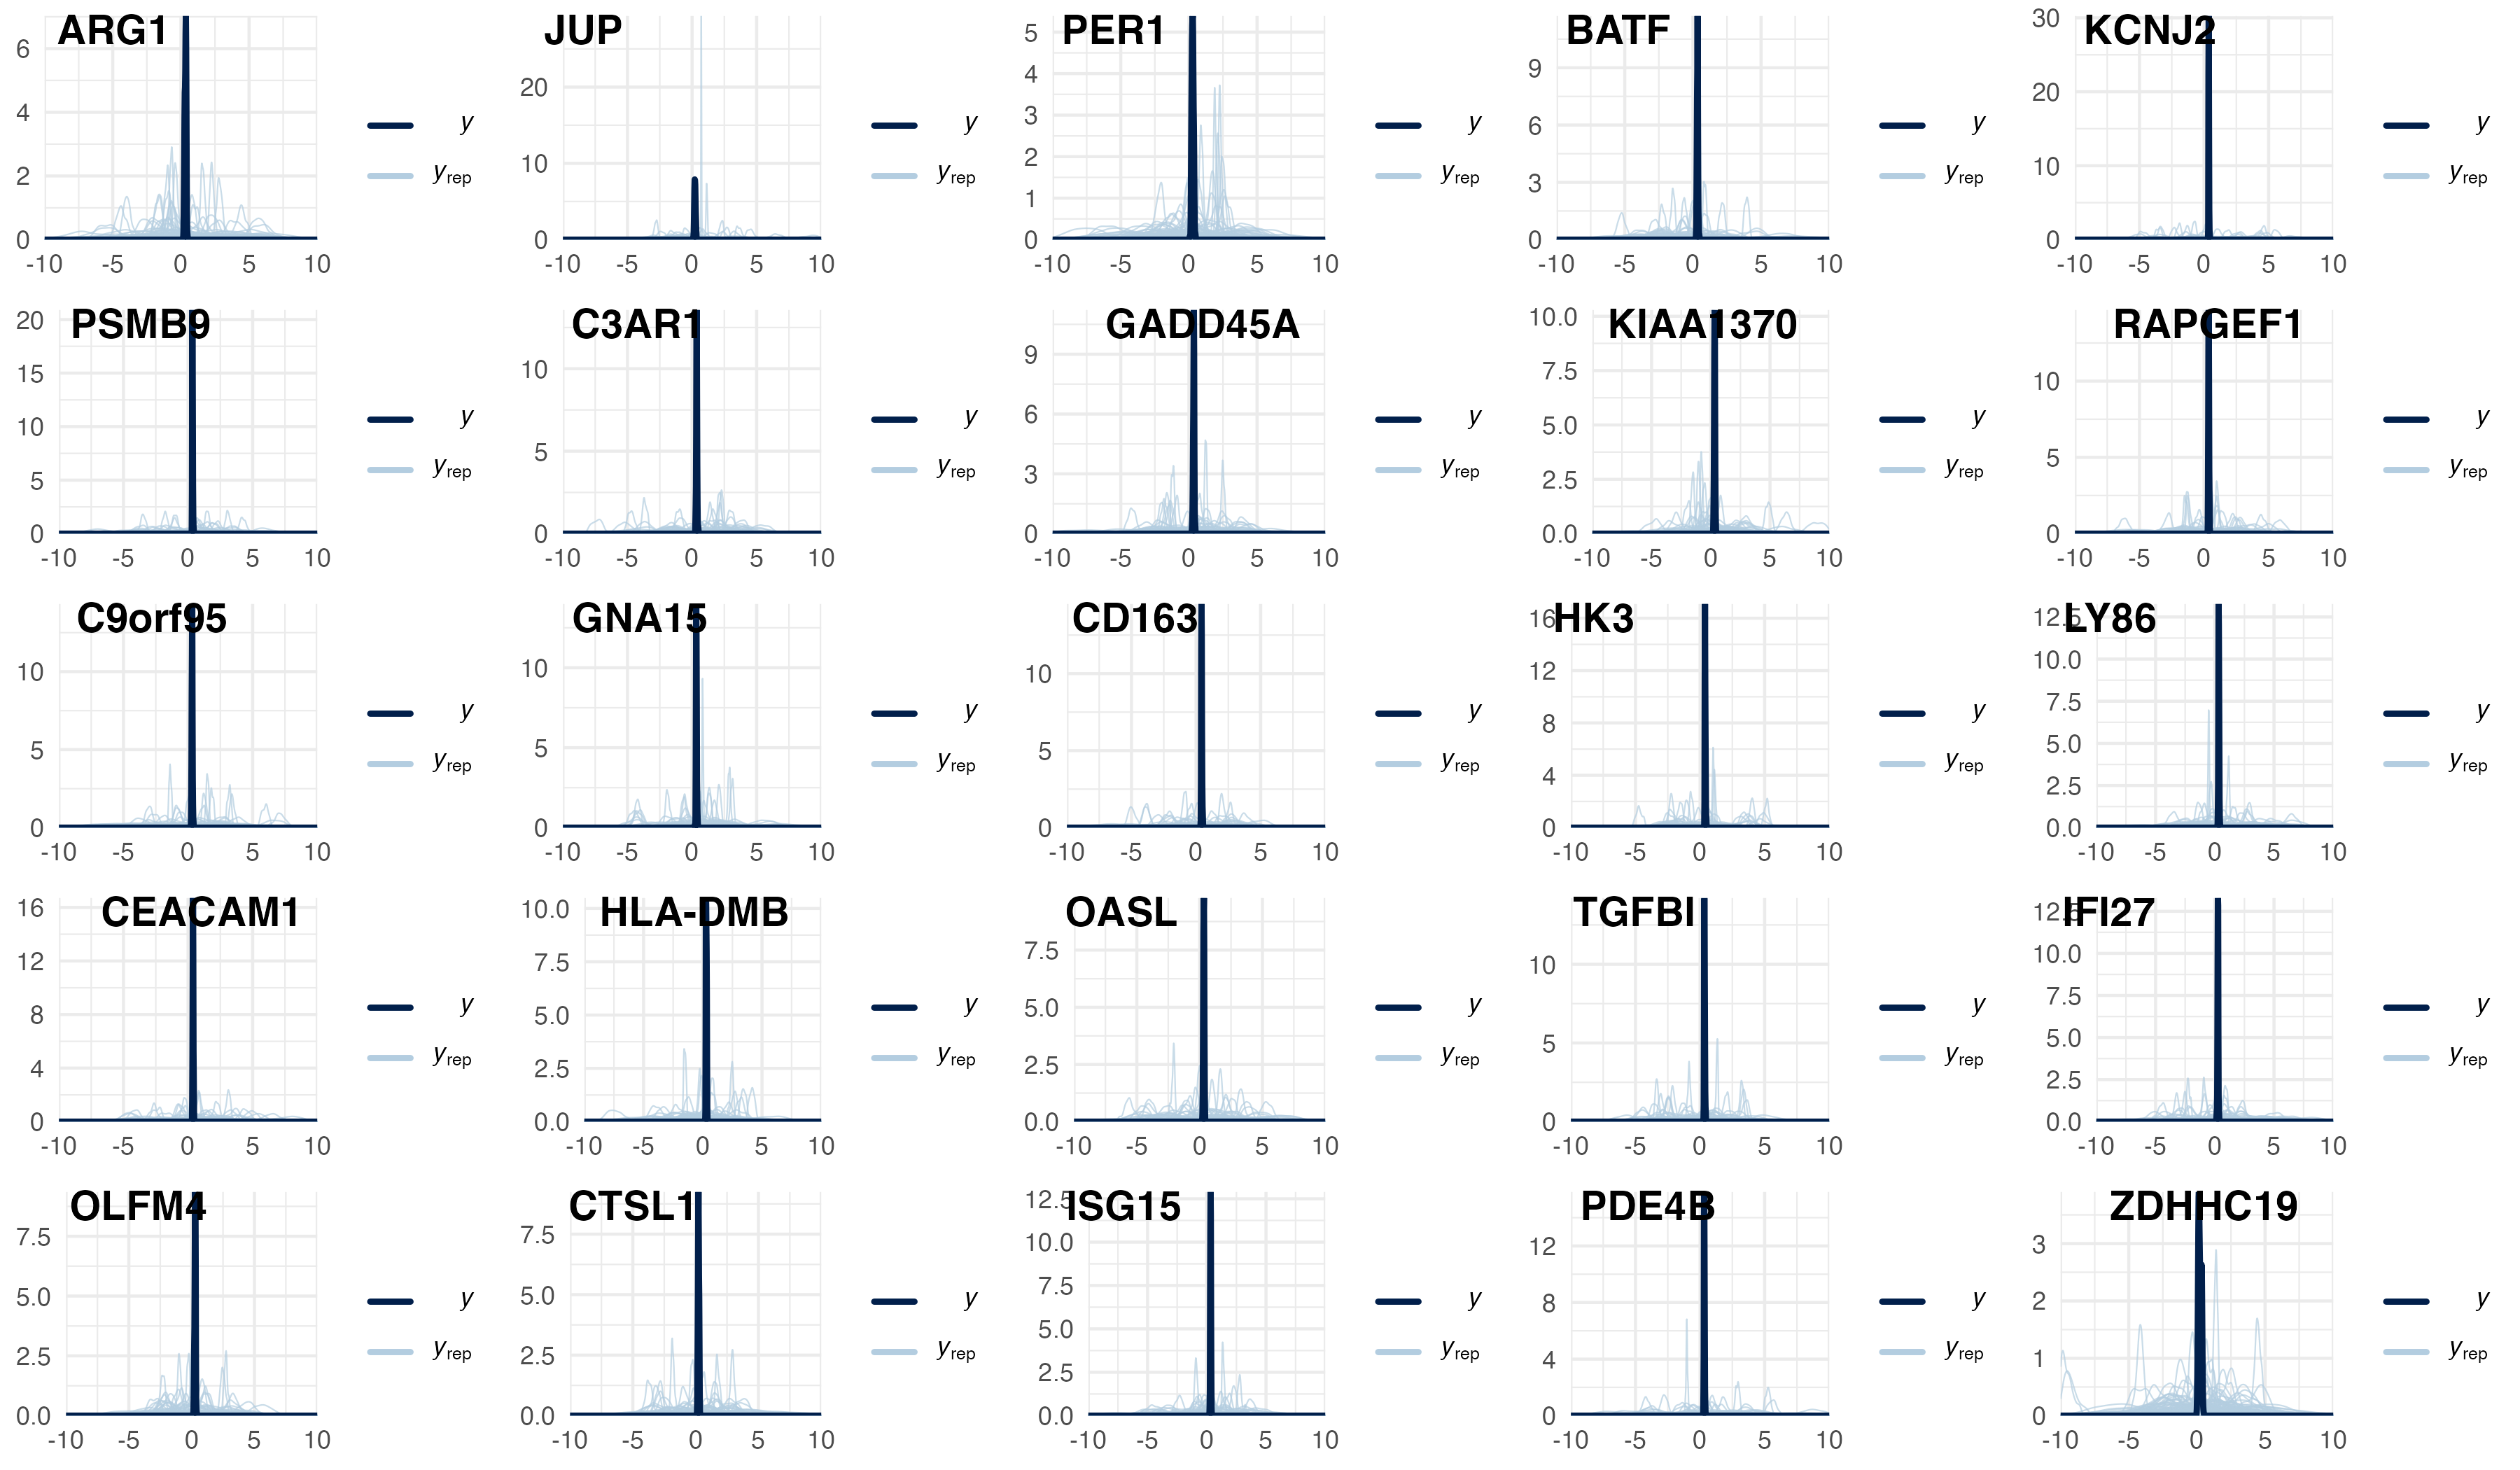
\includegraphics[width=\textwidth]{figures/chapter2/clinical_single_target_rate_priors_fig.png}
    \caption{Prior predictive plots for each of the 25 single-target models fitted of rate $\hat{B}_{ij}$, summarised in Table~\ref{tab:single_target_rate_models_summary} in the main text.}
    \label{fig:clinical_single_target_rate_priors_fig}
\end{figure}

\begin{figure}[!ht]
    \centering
    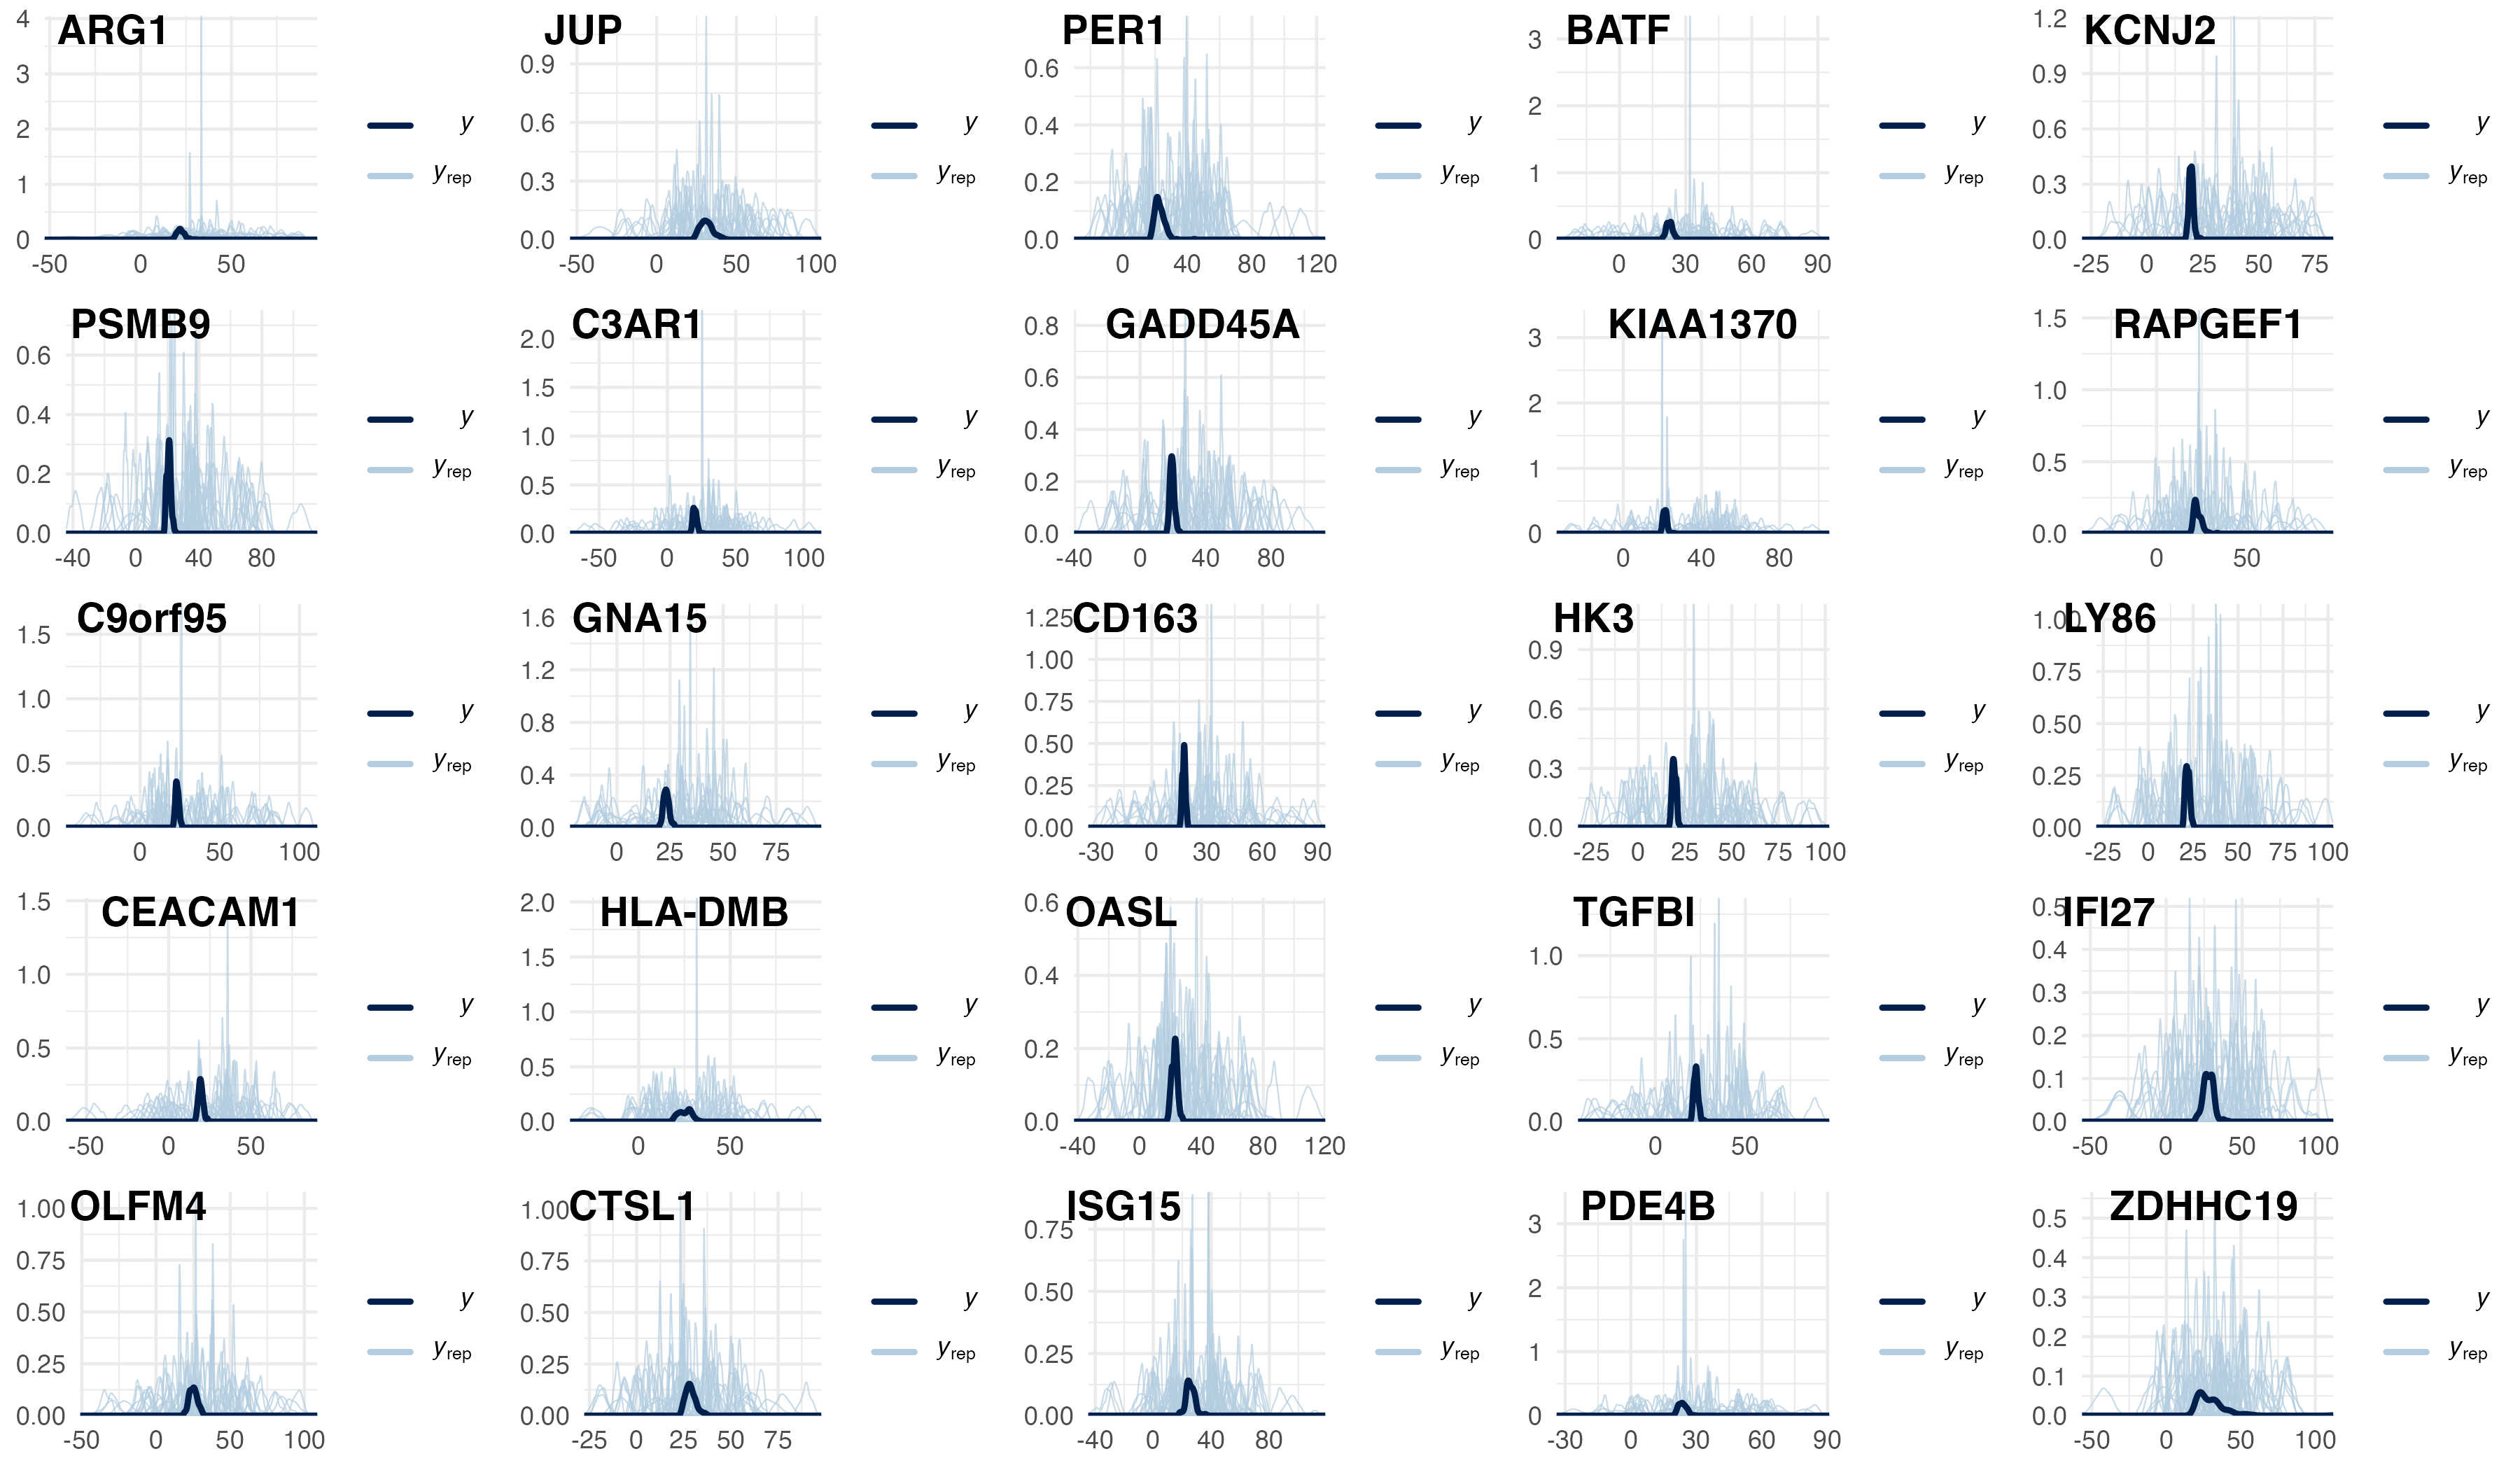
\includegraphics[width=\textwidth]{figures/chapter2/clinical_single_target_offset_priors_fig.png}
    \caption{Prior predictive plots for each of the 25 single-target models fitted of offset $\hat{C}_{ij}$, summarised in Table~\ref{tab:single_target_offset_models_summary} in the main text.}
    \label{fig:clinical_single_target_offset_priors_fig}
\end{figure}





\newpage
\newpage
\section{Posterior Checks}
We next give posterior predictive check plots for the same set of 25 models. These, rather than simply aiming to show a distribution encompassing the range of the observed distribution, aim to show a fitted distribution that closely matches it. Once again, we show posterior summaries for models of rate (Figure~\ref{fig:clinical_single_target_rate_posteriors_fig}) and of cycle offset (Figure~\ref{fig:clinical_single_target_offset_posteriors_fig}).



\begin{figure}
    \centering
    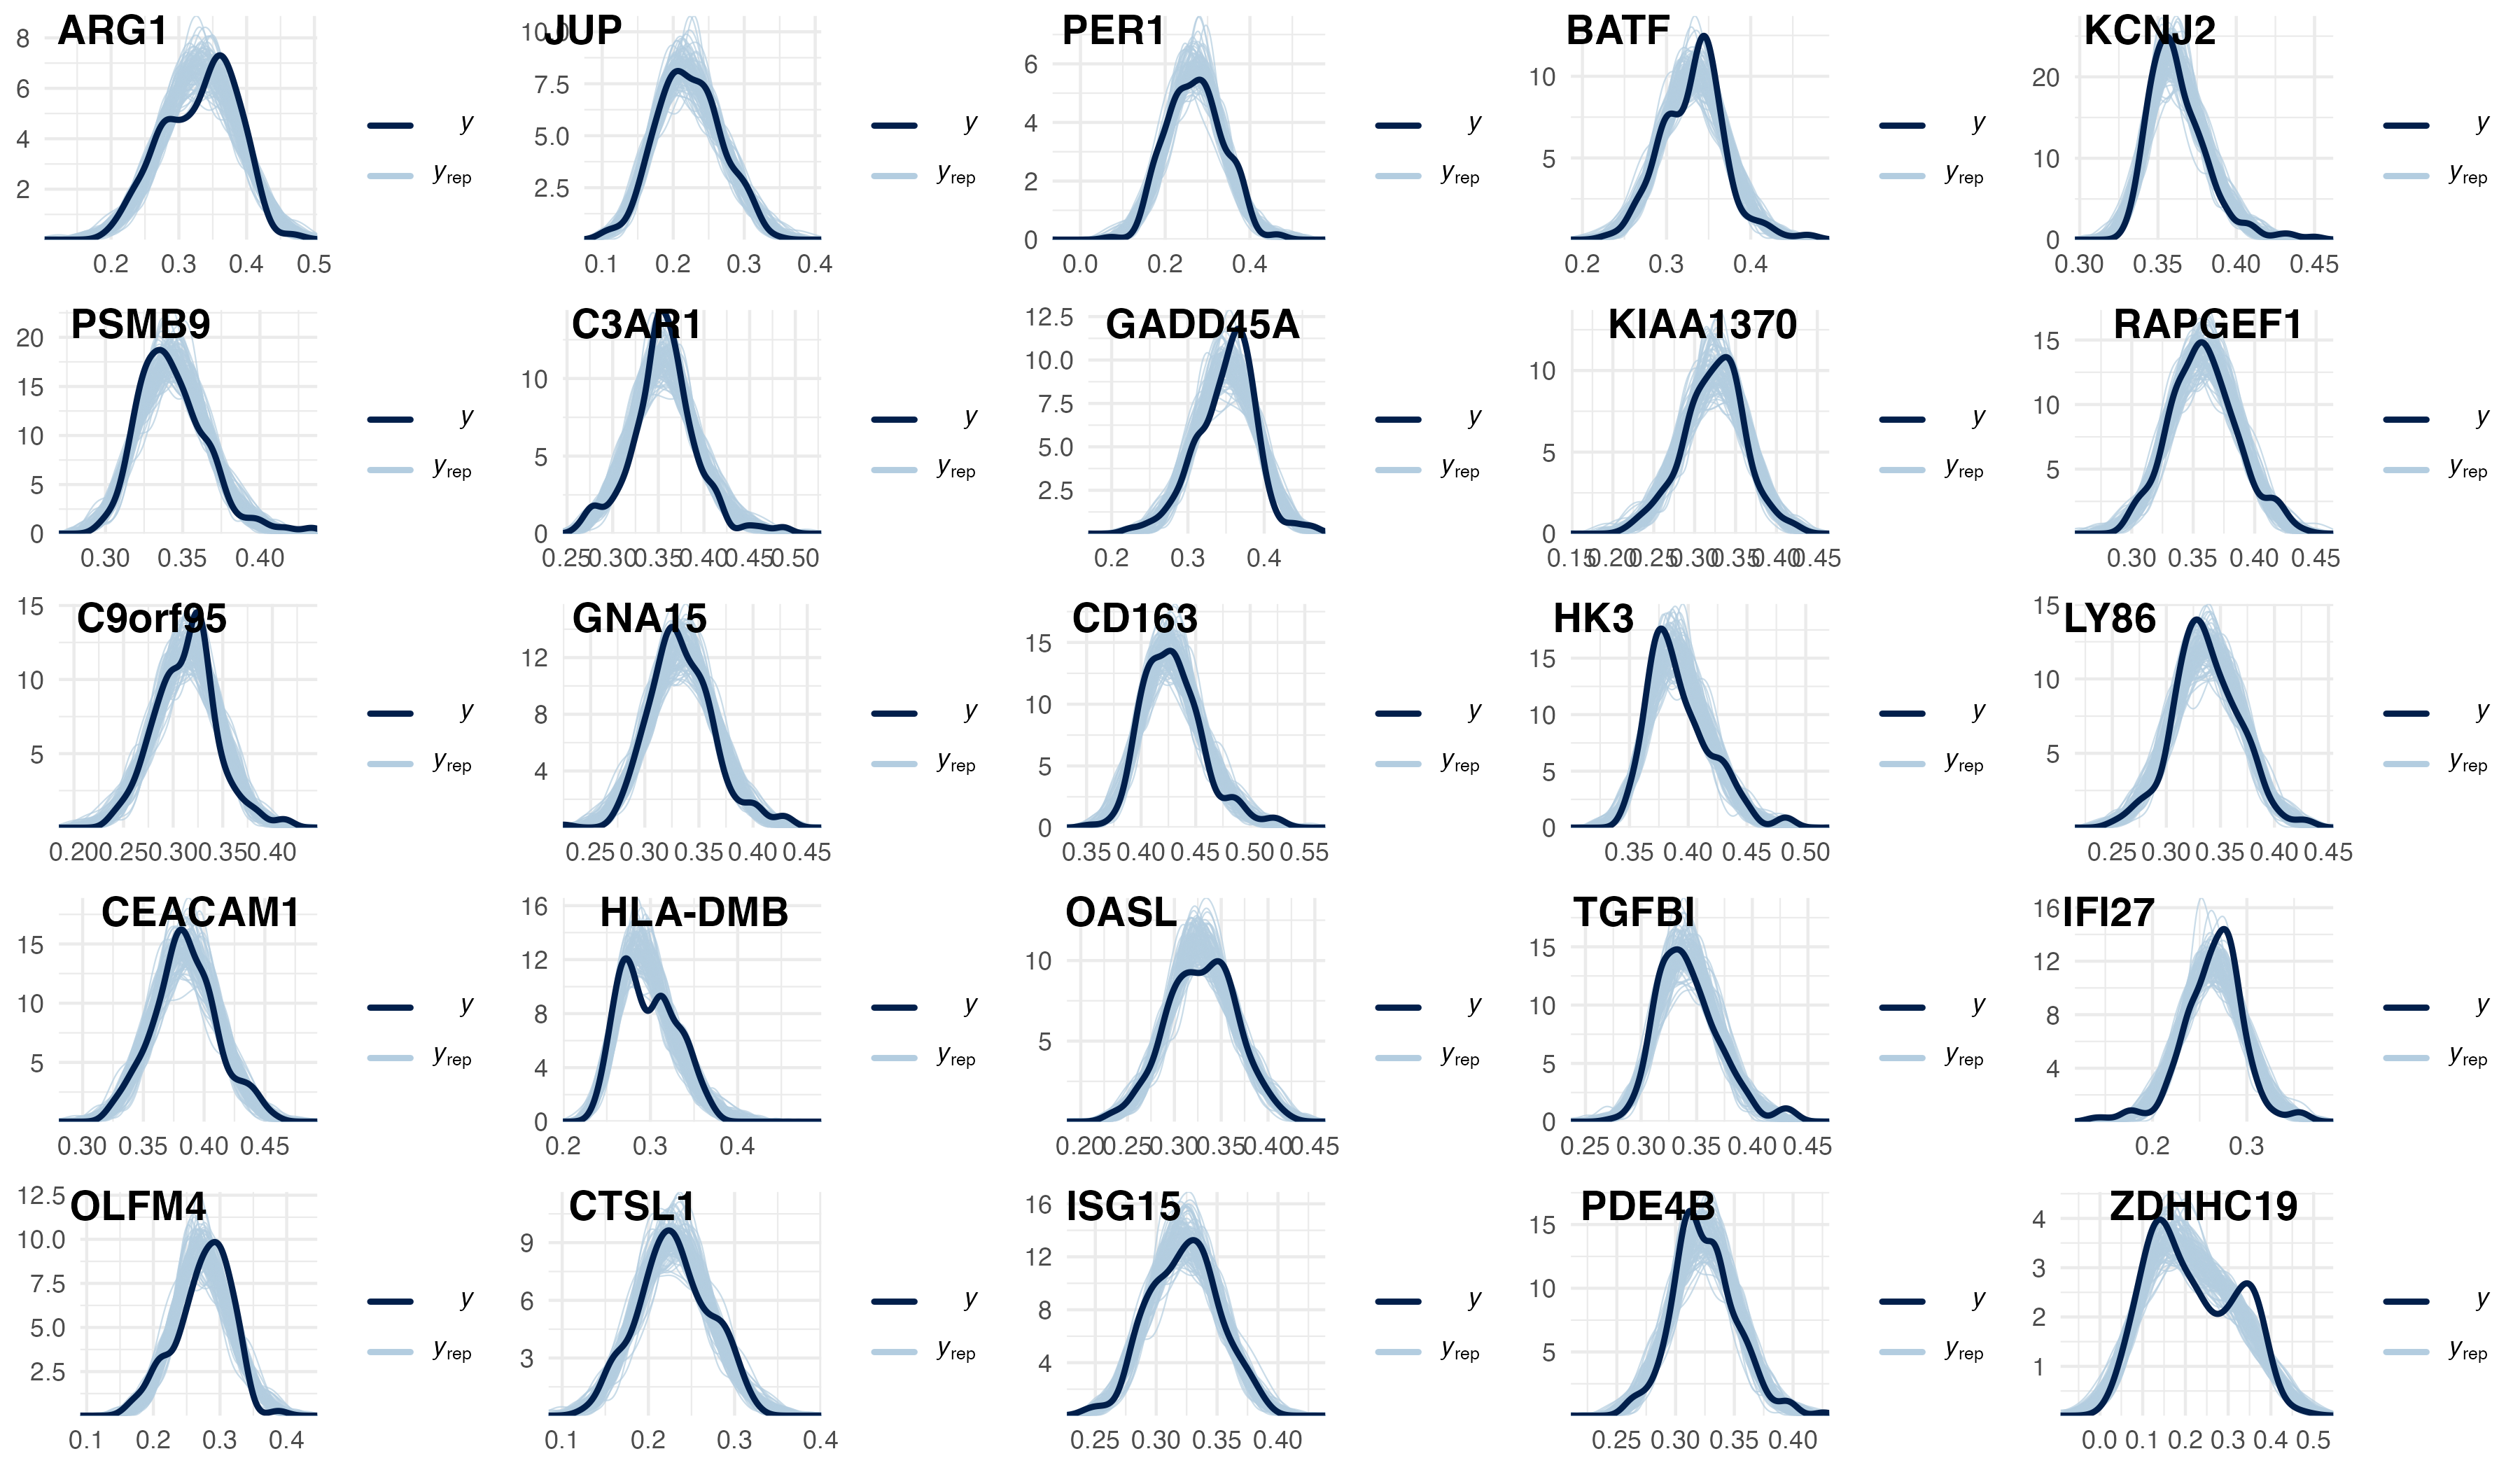
\includegraphics[width=\textwidth]{figures/chapter2/clinical_single_target_rate_posteriors_fig.png}
    \caption{Posterior predictive plots for each of the 25 single-target models fitted of offset $\hat{C}_{ij}$, summarised in Table~\ref{tab:single_target_rate_models_summary} in the main text.}
    \label{fig:clinical_single_target_rate_posteriors_fig}
\end{figure}

\begin{figure}[!ht]
    \centering
    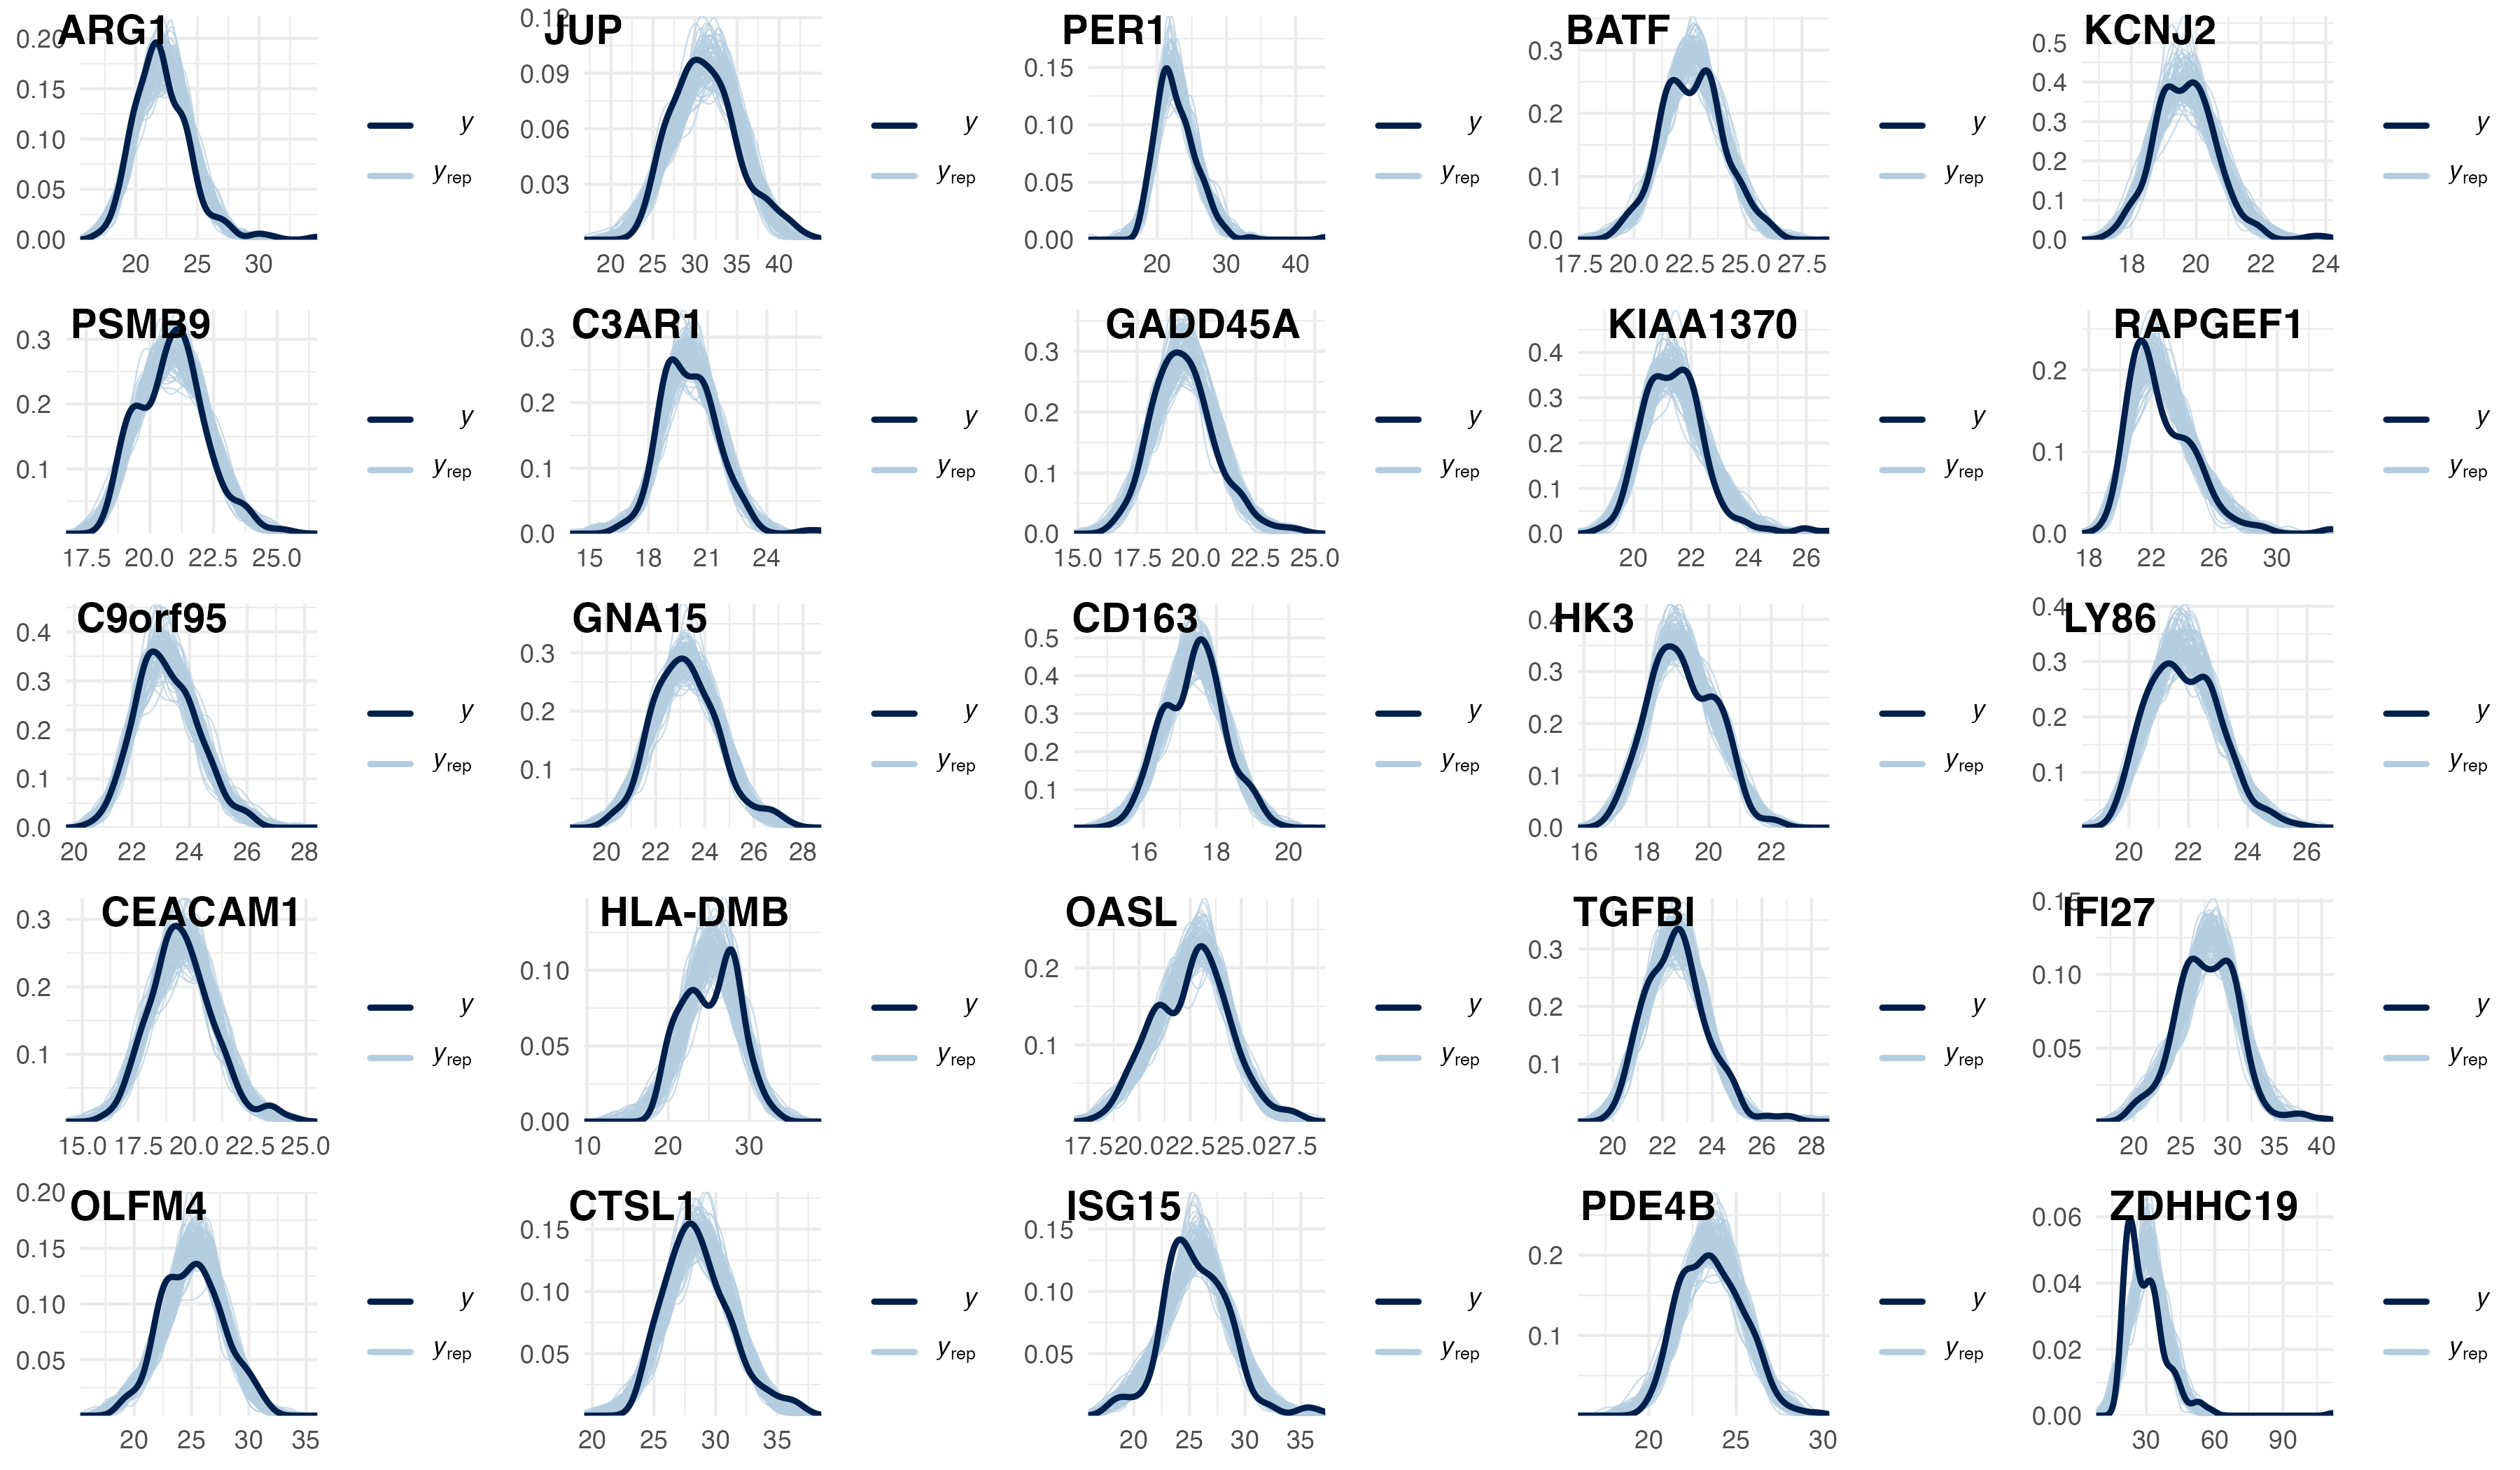
\includegraphics[width=\textwidth]{figures/chapter2/clinical_single_target_offset_posteriors_fig.png}
    \caption{Posterior predictive plots for each of the 25 single-target models fitted of offset $\hat{C}_{ij}$, summarised in Table~\ref{tab:single_target_offset_models_summary} in the main text.}
    \label{fig:clinical_single_target_offset_posteriors_fig}
\end{figure}

\newpage
\section{Model Convergence}
Finally, we present \gls{hmc} convergence summaries for each of the 25 single-target models of both rate and cycle offset.
\begin{figure}[!hb]
    \centering
    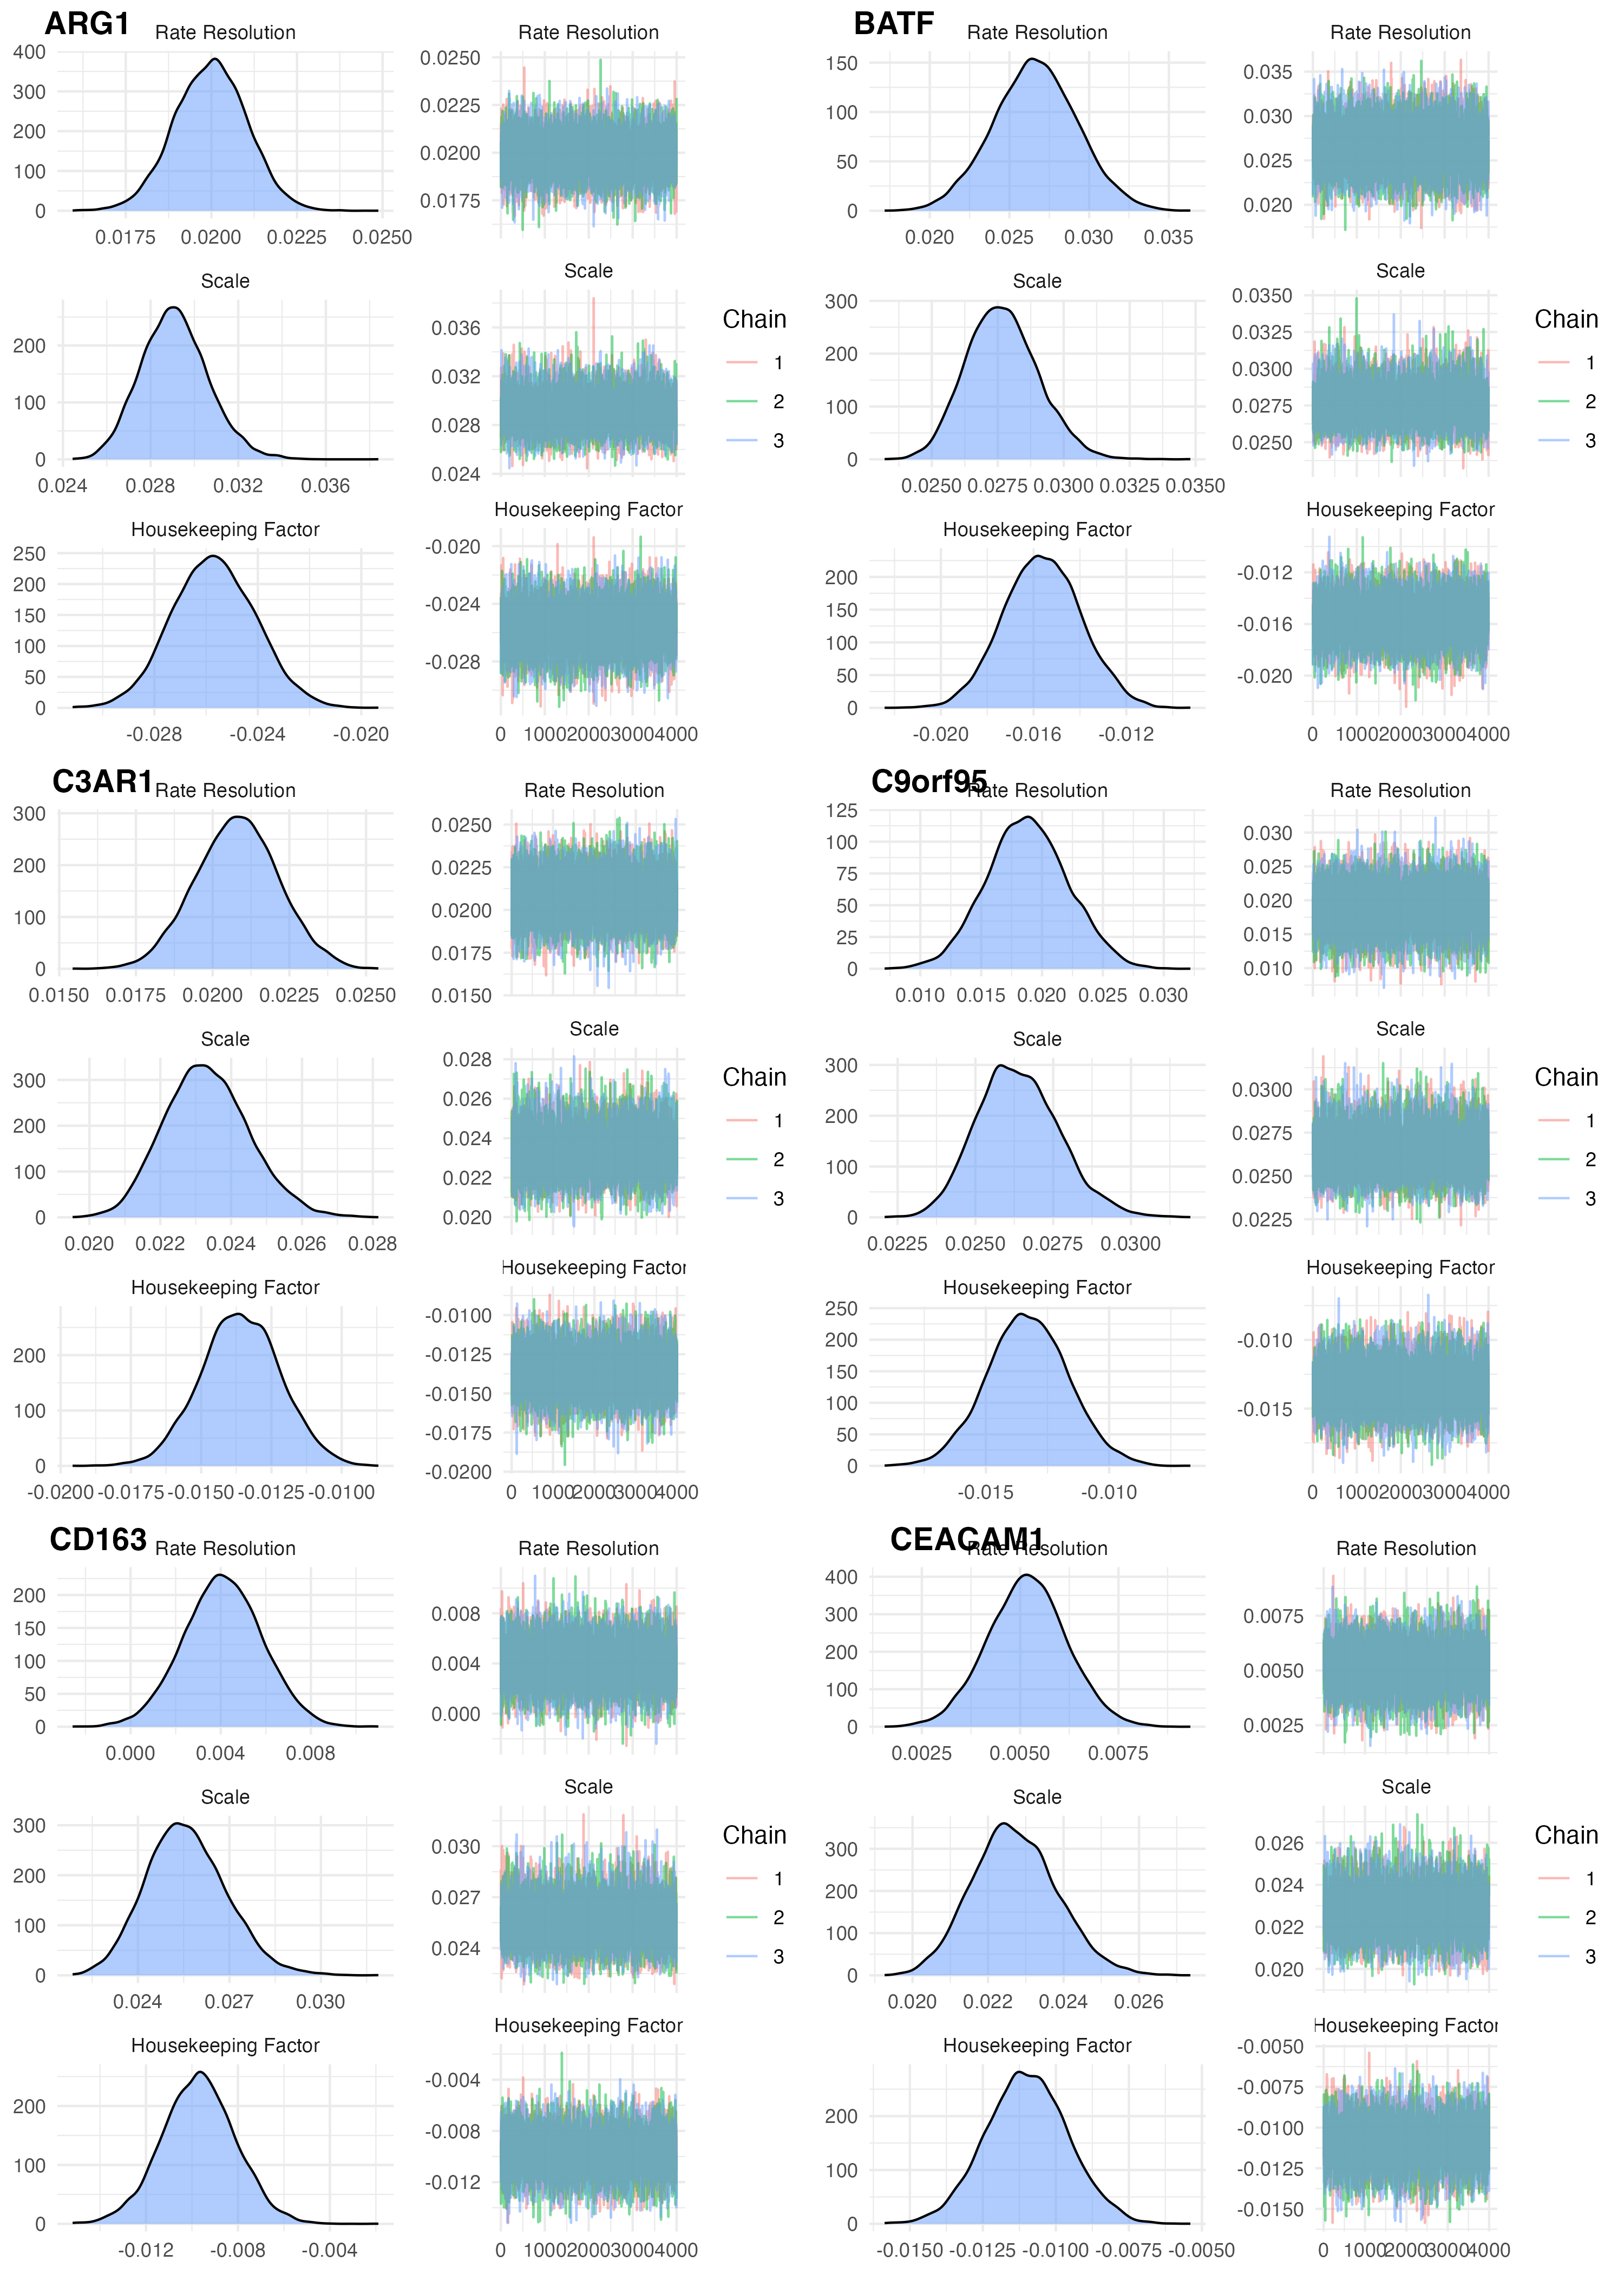
\includegraphics[width=\textwidth]{figures/chapter2/model_summaries_5.png}
    \caption{Model convergence summaries for each of the 25 single-target rate models summarised in Table~\ref{tab:single_target_rate_models_summary}.}
    \label{fig:convergence_5}
\end{figure}

\begin{figure}
    \centering
    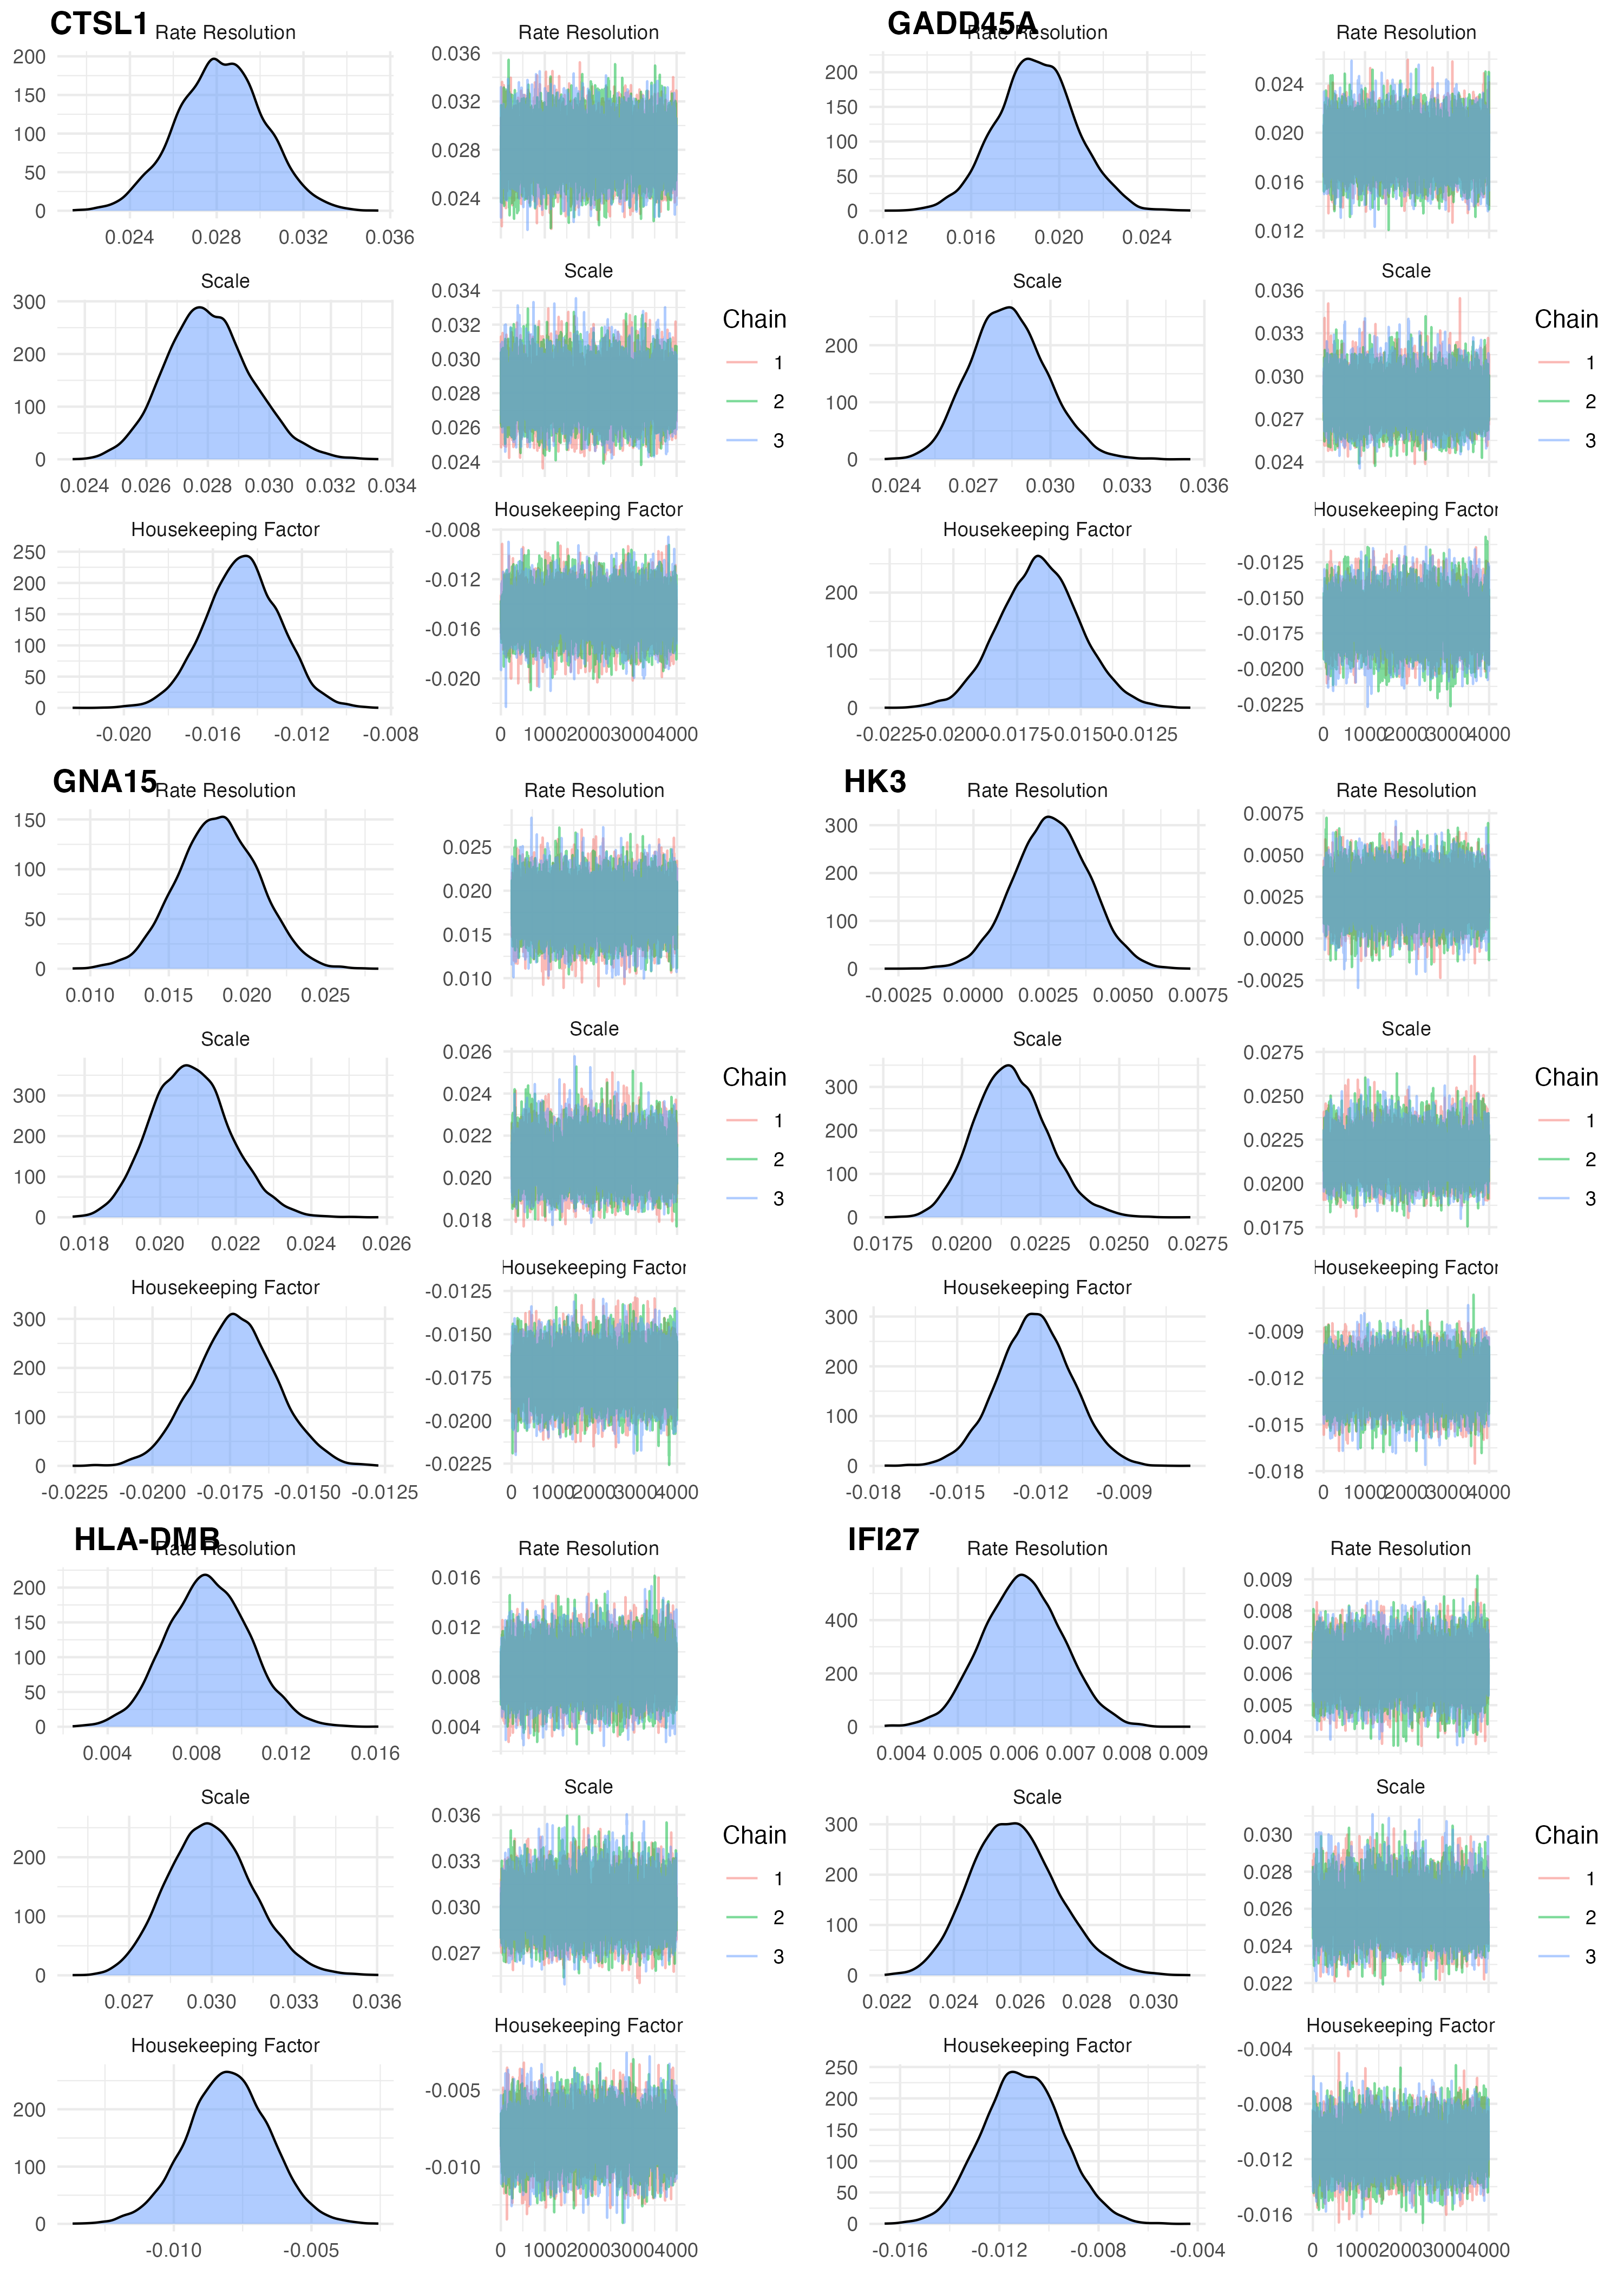
\includegraphics[width=\textwidth]{figures/chapter2/model_summaries_6.png}
    \caption{Model convergence summaries for each of the 25 single-target rate models summarised in Table~\ref{tab:single_target_rate_models_summary} (continued).}
    \label{fig:convergence_6}
\end{figure}

\begin{figure}
    \centering
    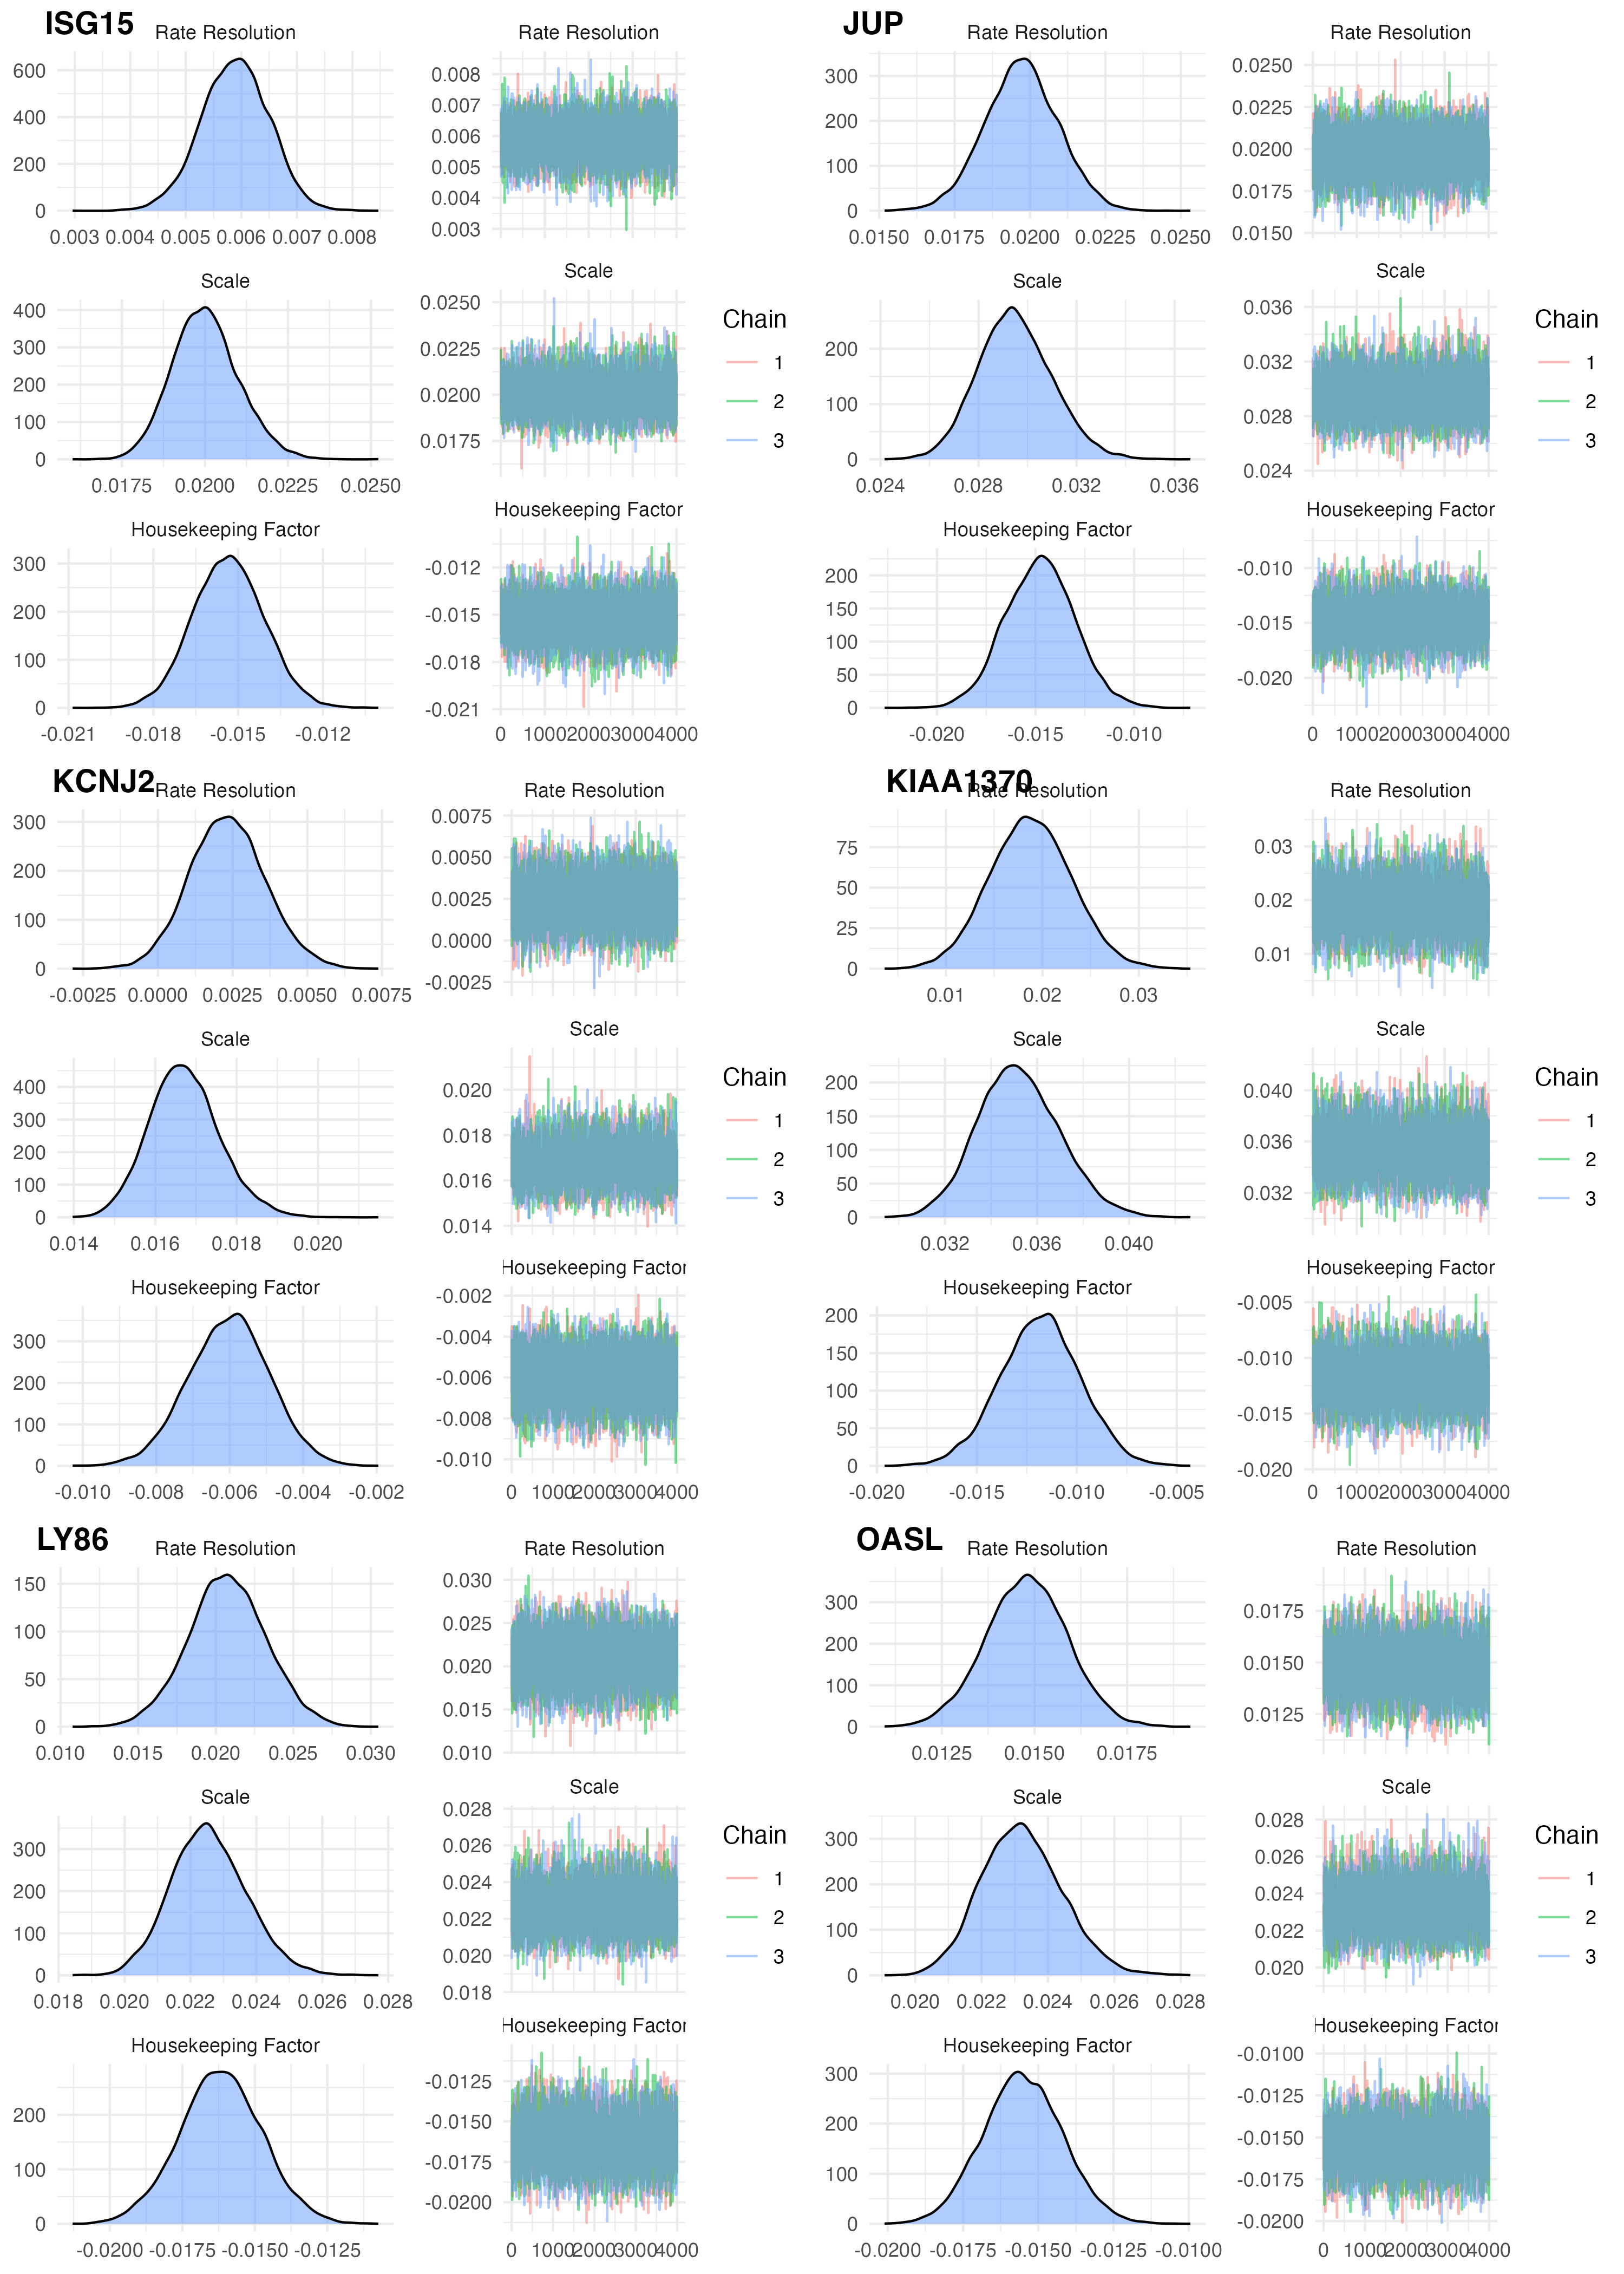
\includegraphics[width=\textwidth]{figures/chapter2/model_summaries_7.png}
    \caption{Model convergence summaries for each of the 25 single-target rate models summarised in Table~\ref{tab:single_target_rate_models_summary} (continued).}
    \label{fig:convergence_7}
\end{figure}

\begin{figure}
    \centering
    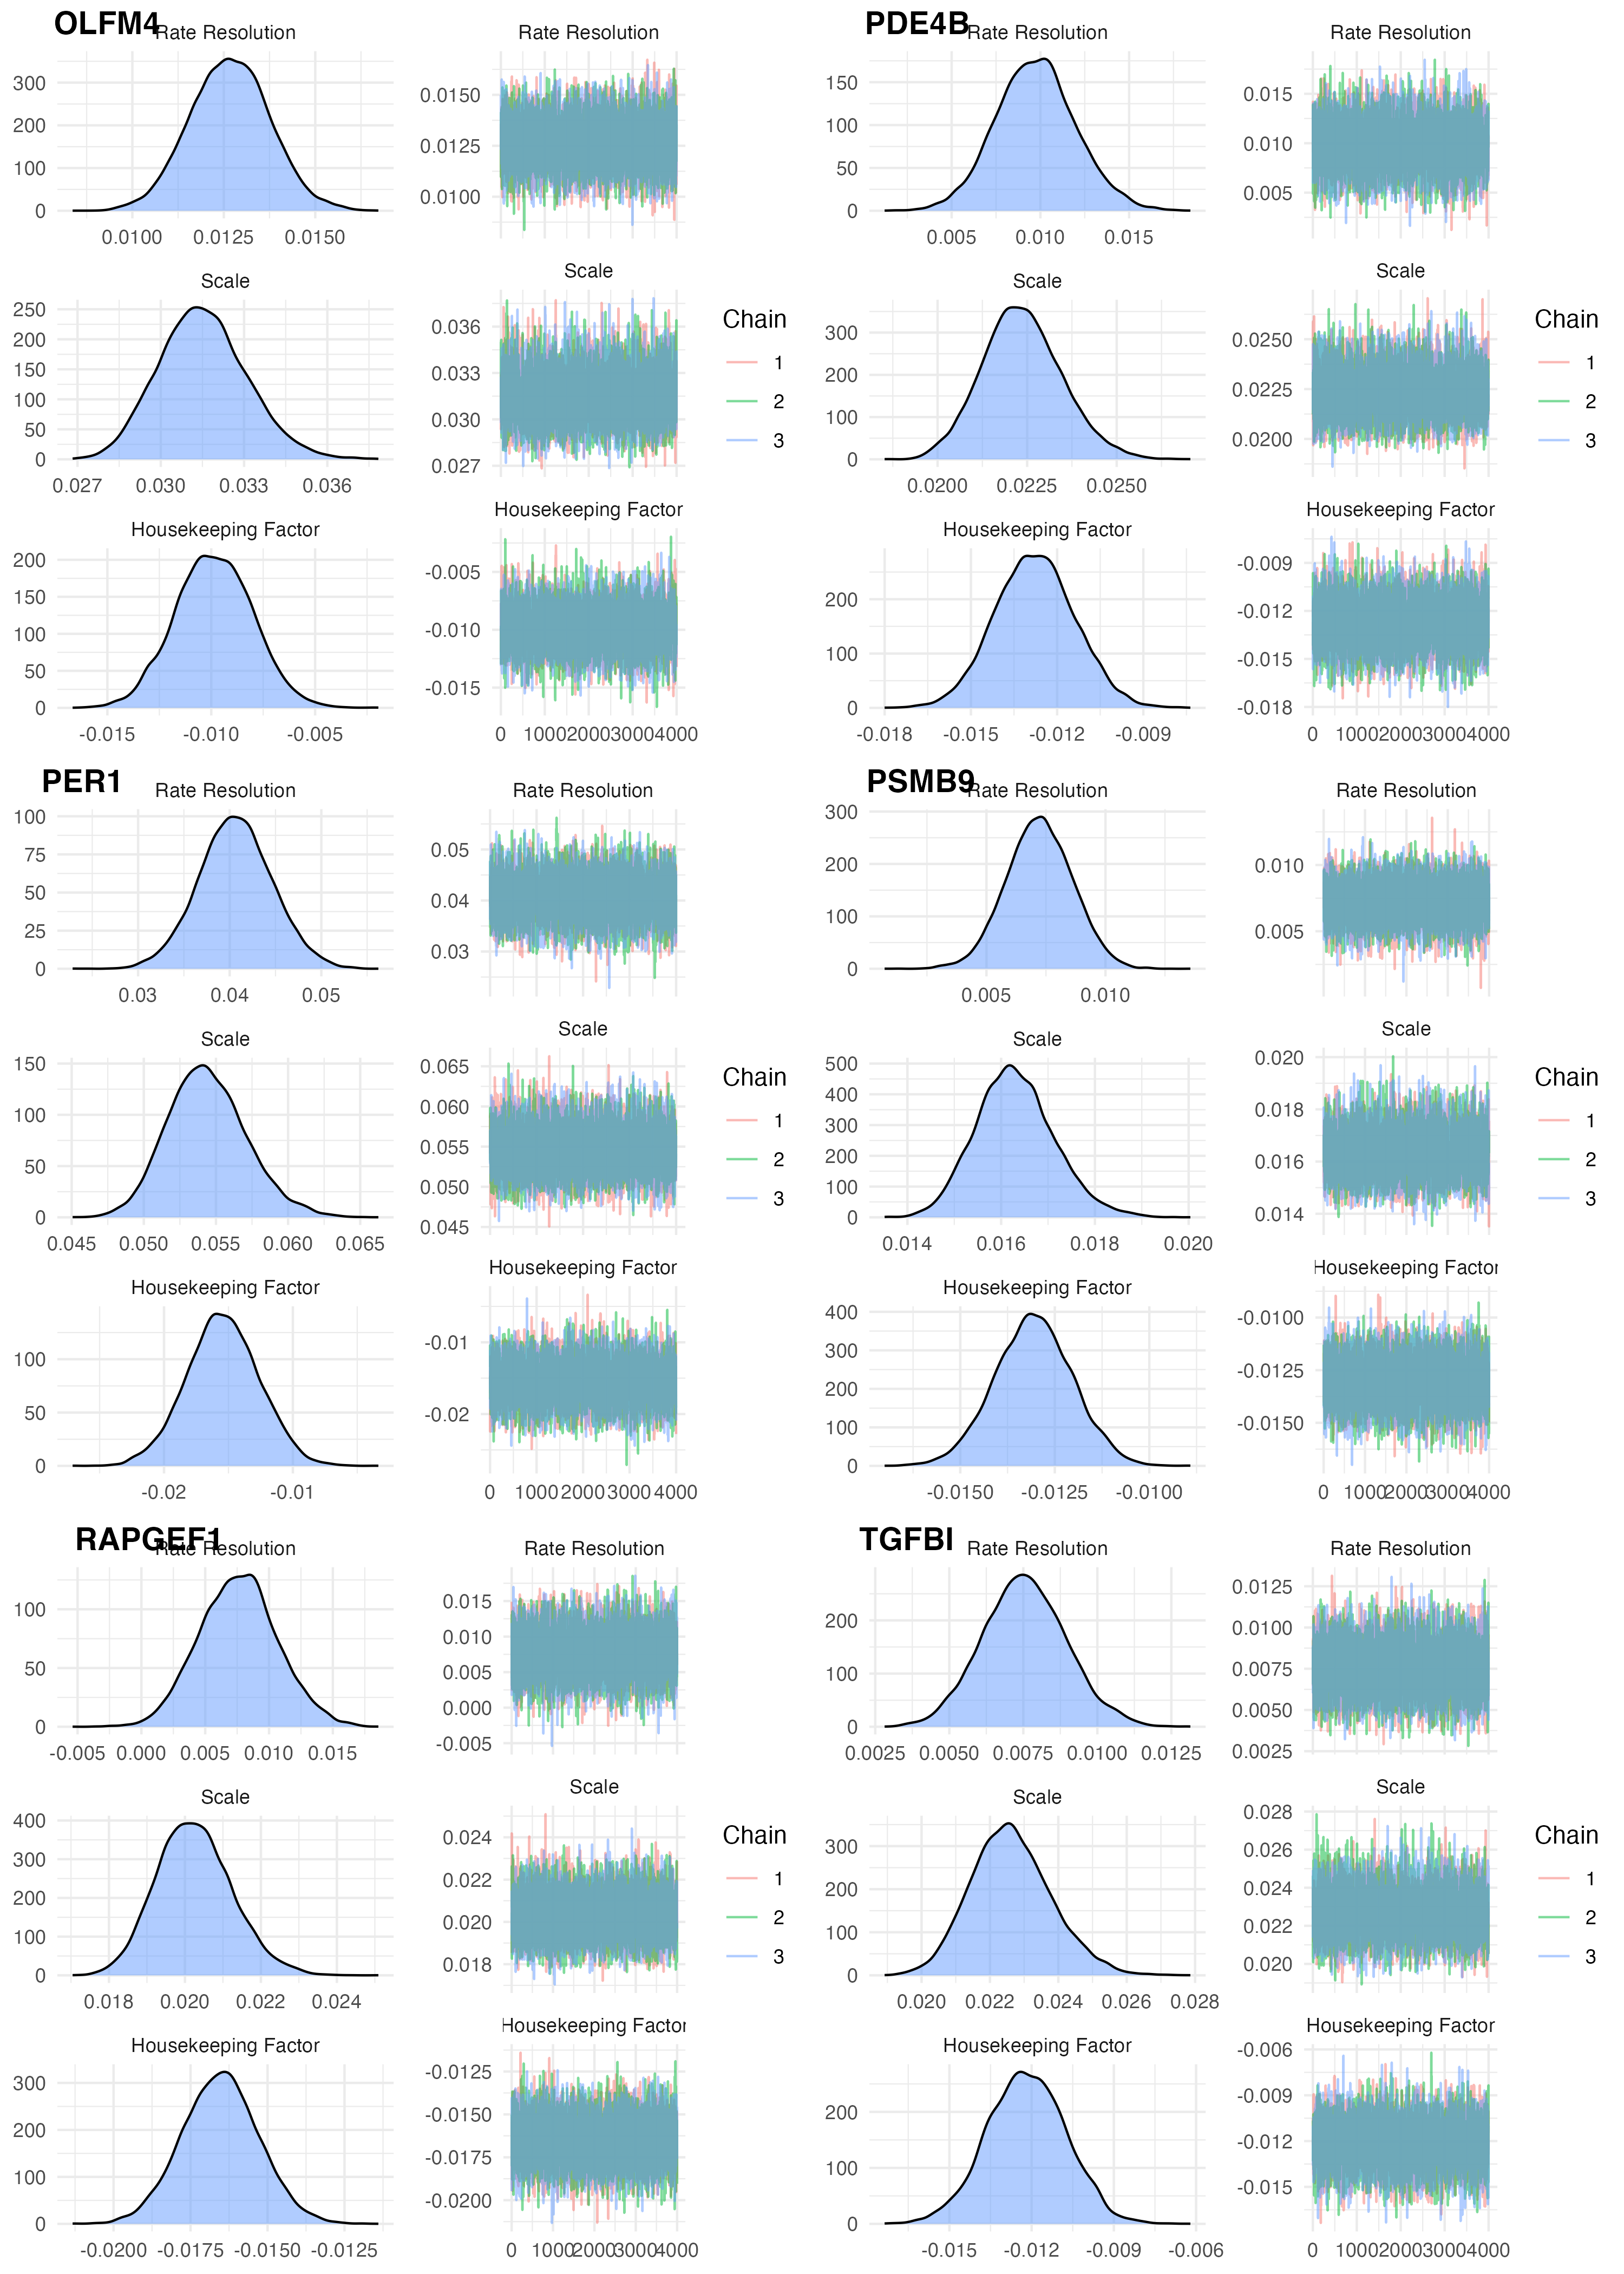
\includegraphics[width=\textwidth]{figures/chapter2/model_summaries_8.png}
    \caption{Model convergence summaries for each of the 25 single-target rate models summarised in Table~\ref{tab:single_target_rate_models_summary} (continued).}
    \label{fig:convergence_8}
\end{figure}

\begin{figure}[!hb]
    \centering
    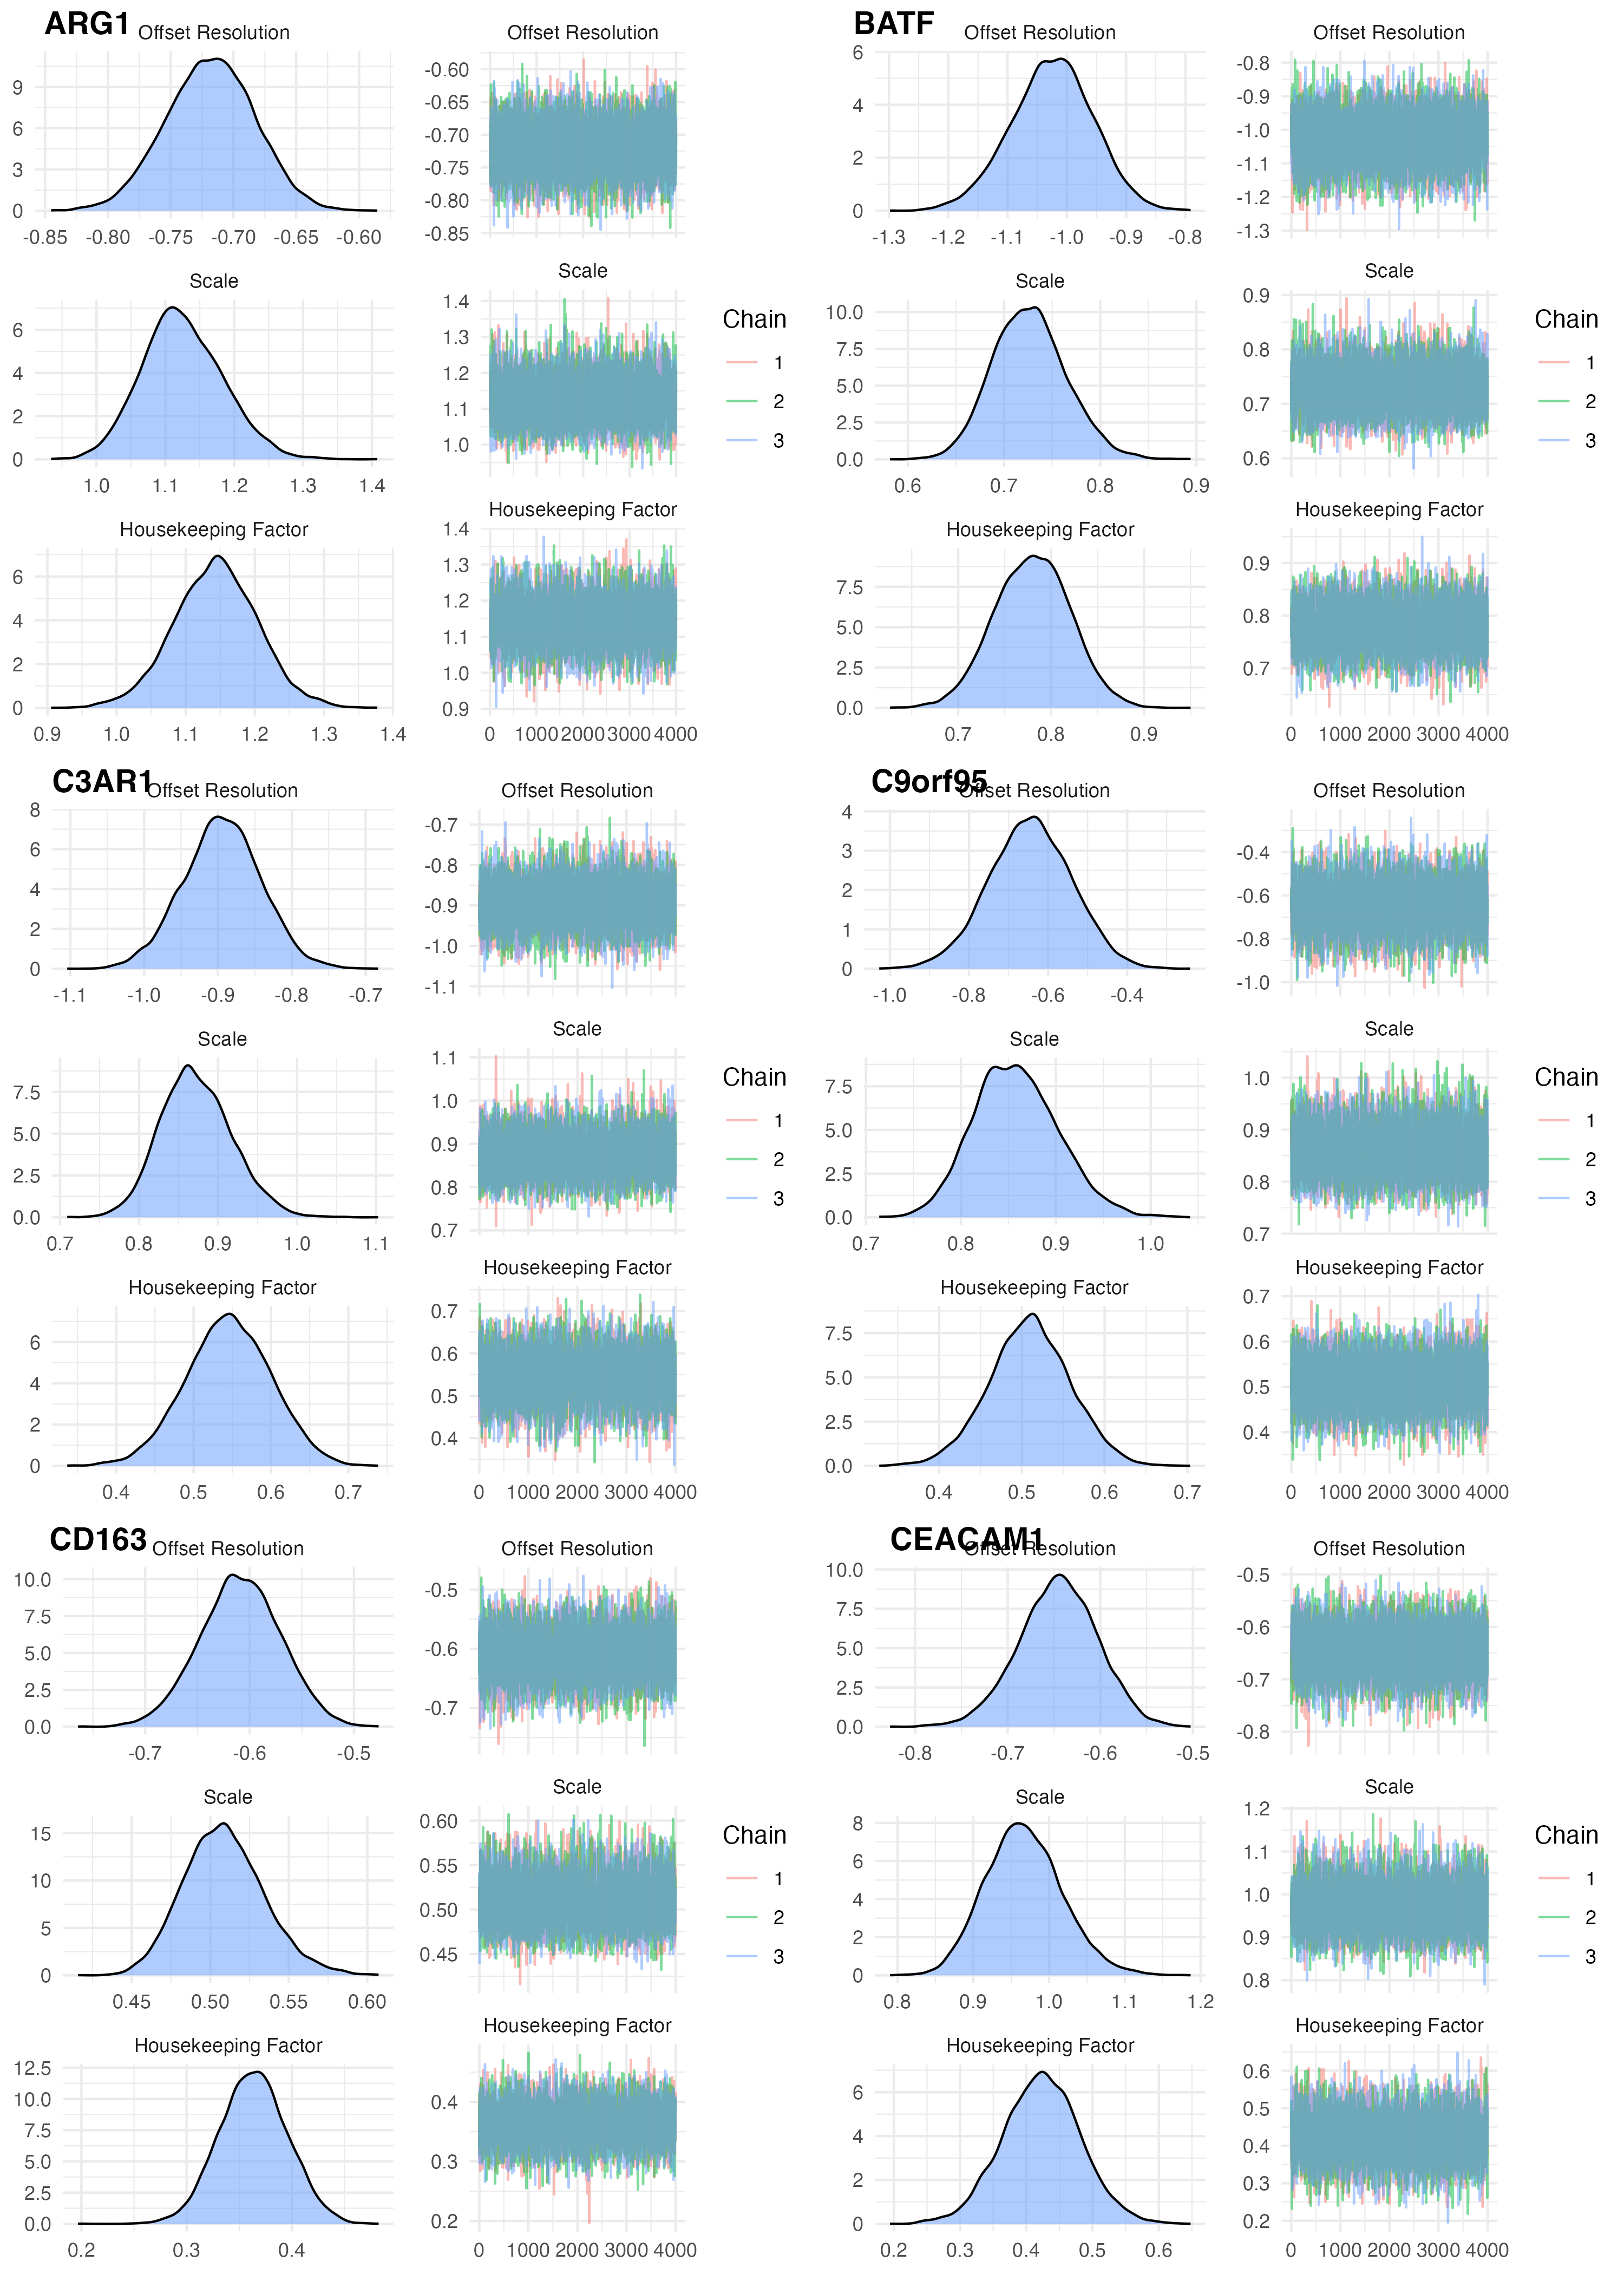
\includegraphics[width=\textwidth]{figures/chapter2/model_summaries_1.png}
    \caption{Model convergence summaries for each of the 25 single-target offset models summarised in Table~\ref{tab:single_target_offset_models_summary}.}
    \label{fig:convergence_1}
\end{figure}

\begin{figure}
    \centering
    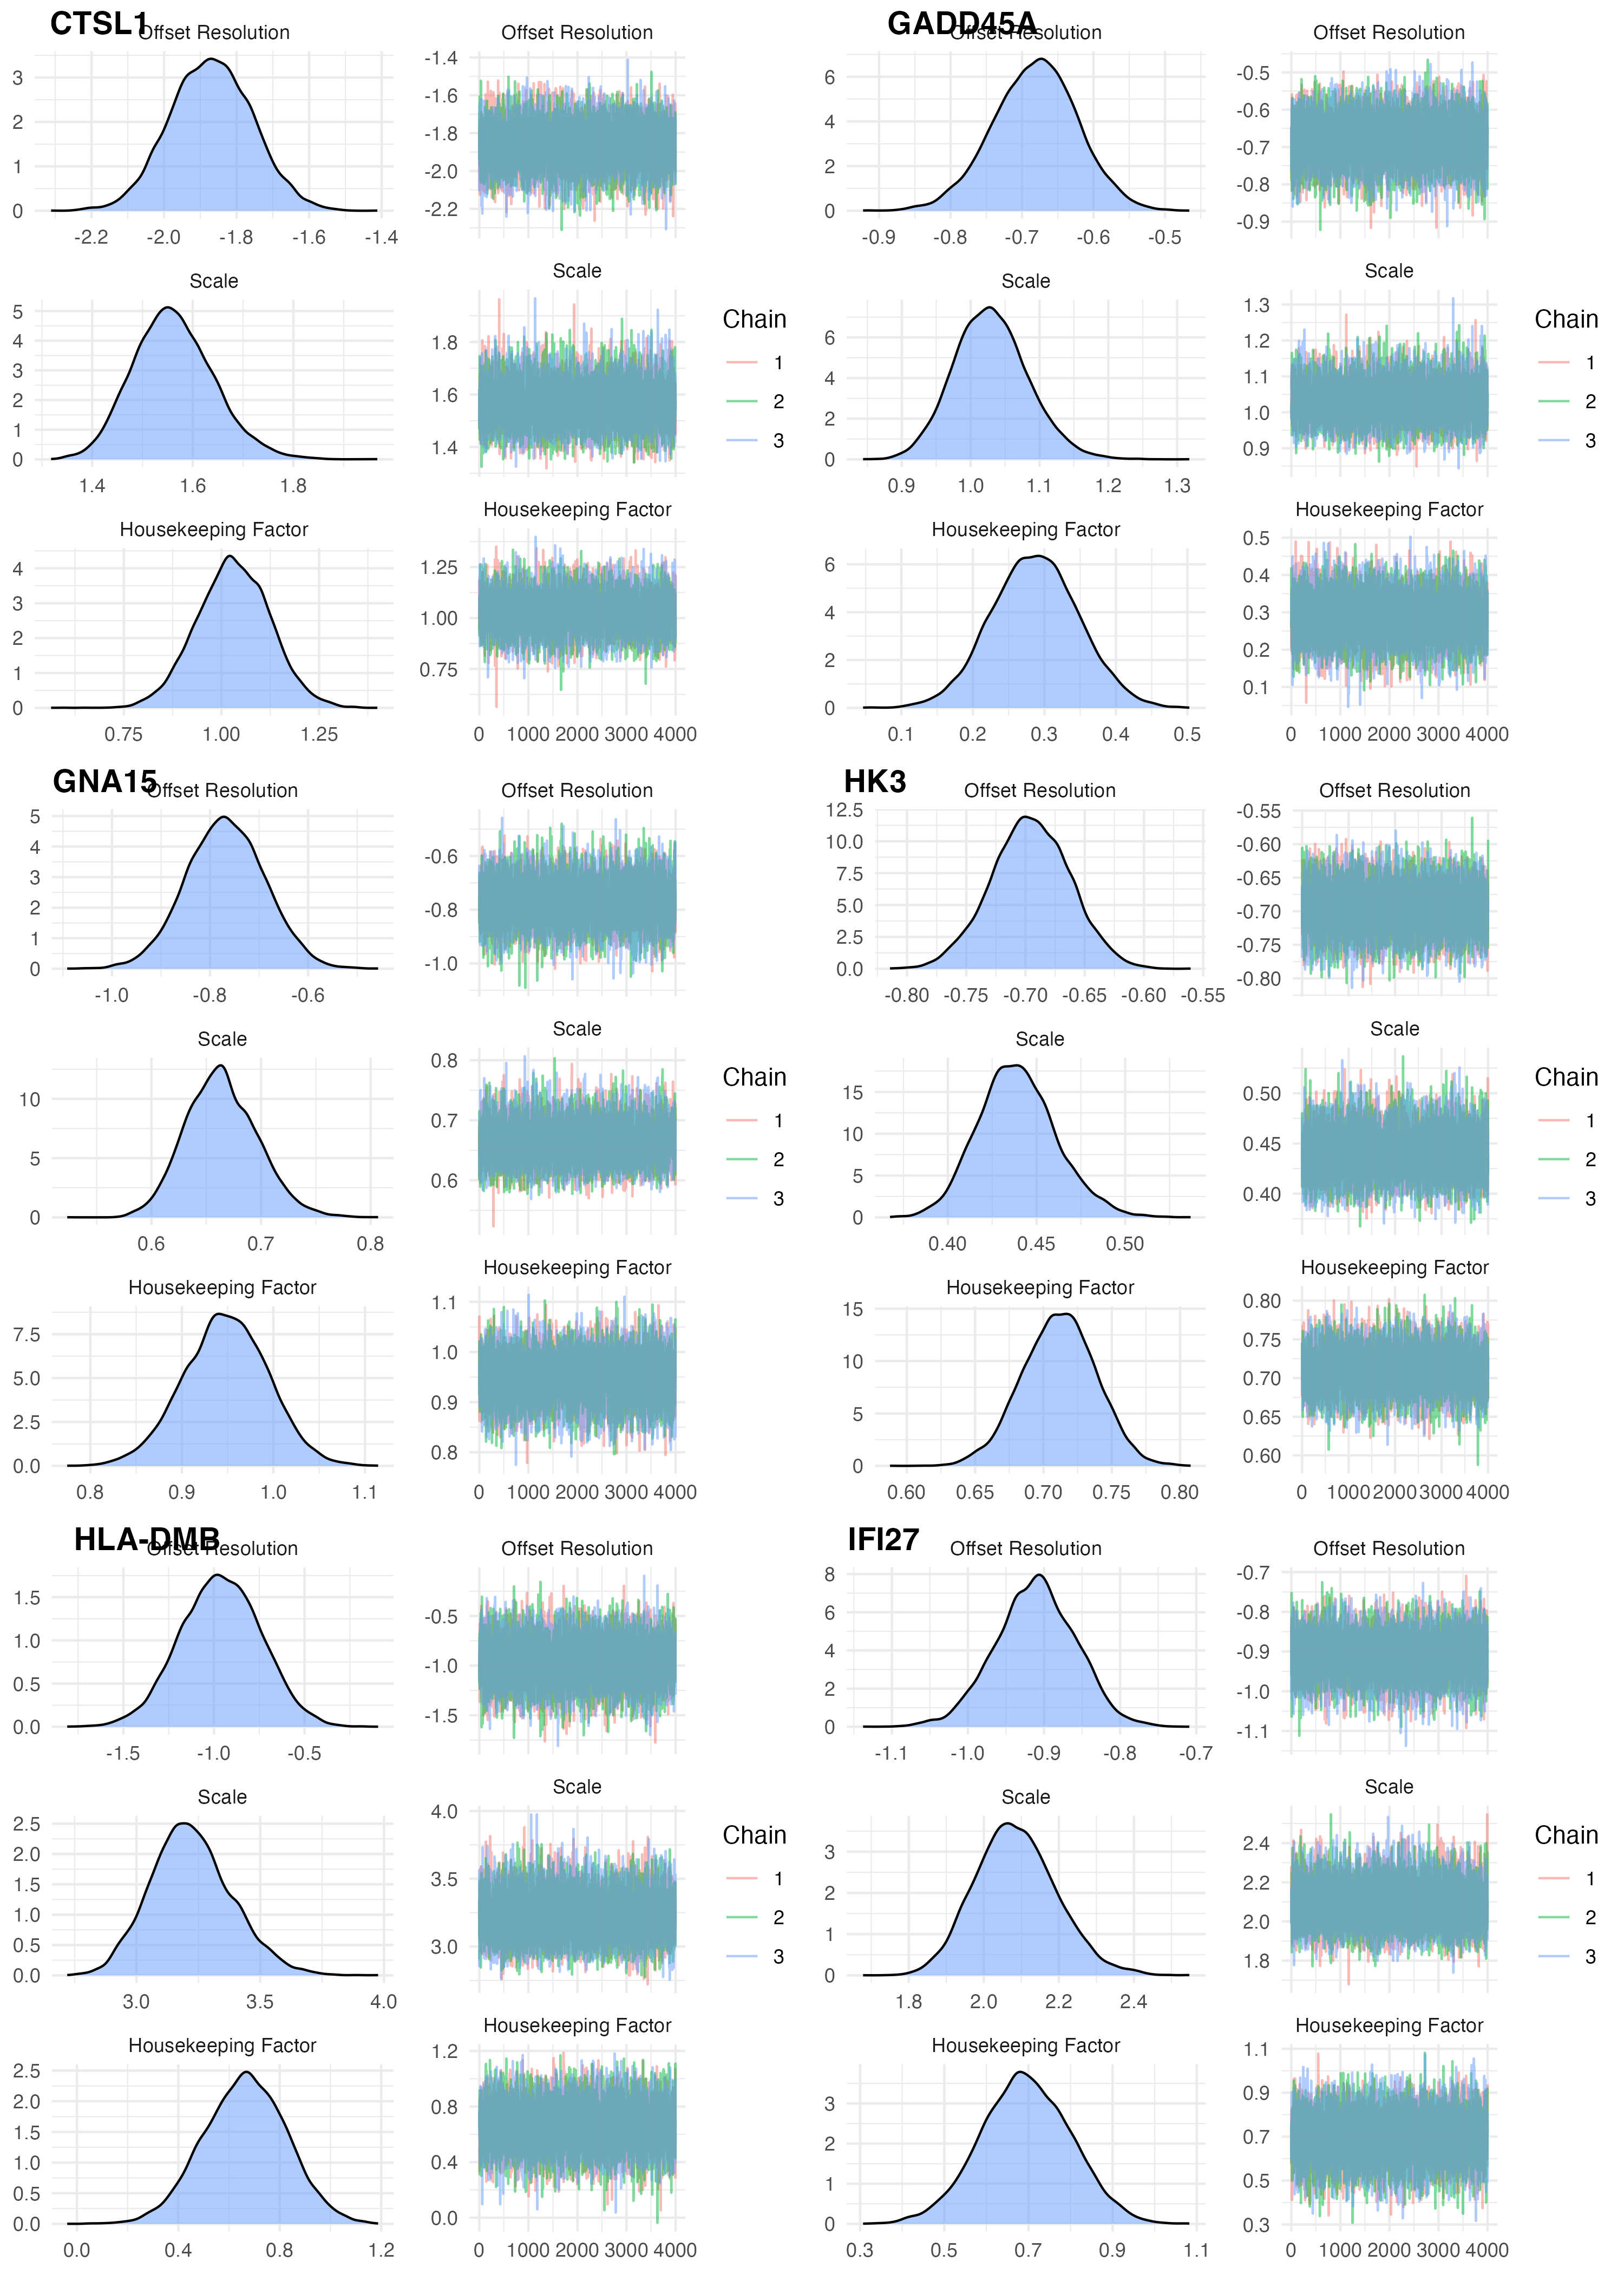
\includegraphics[width=\textwidth]{figures/chapter2/model_summaries_2.png}
    \caption{Model convergence summaries for each of the 25 single-target offset models summarised in Table~\ref{tab:single_target_offset_models_summary} (continued).}
    \label{fig:convergence_2}
\end{figure}

\begin{figure}
    \centering
    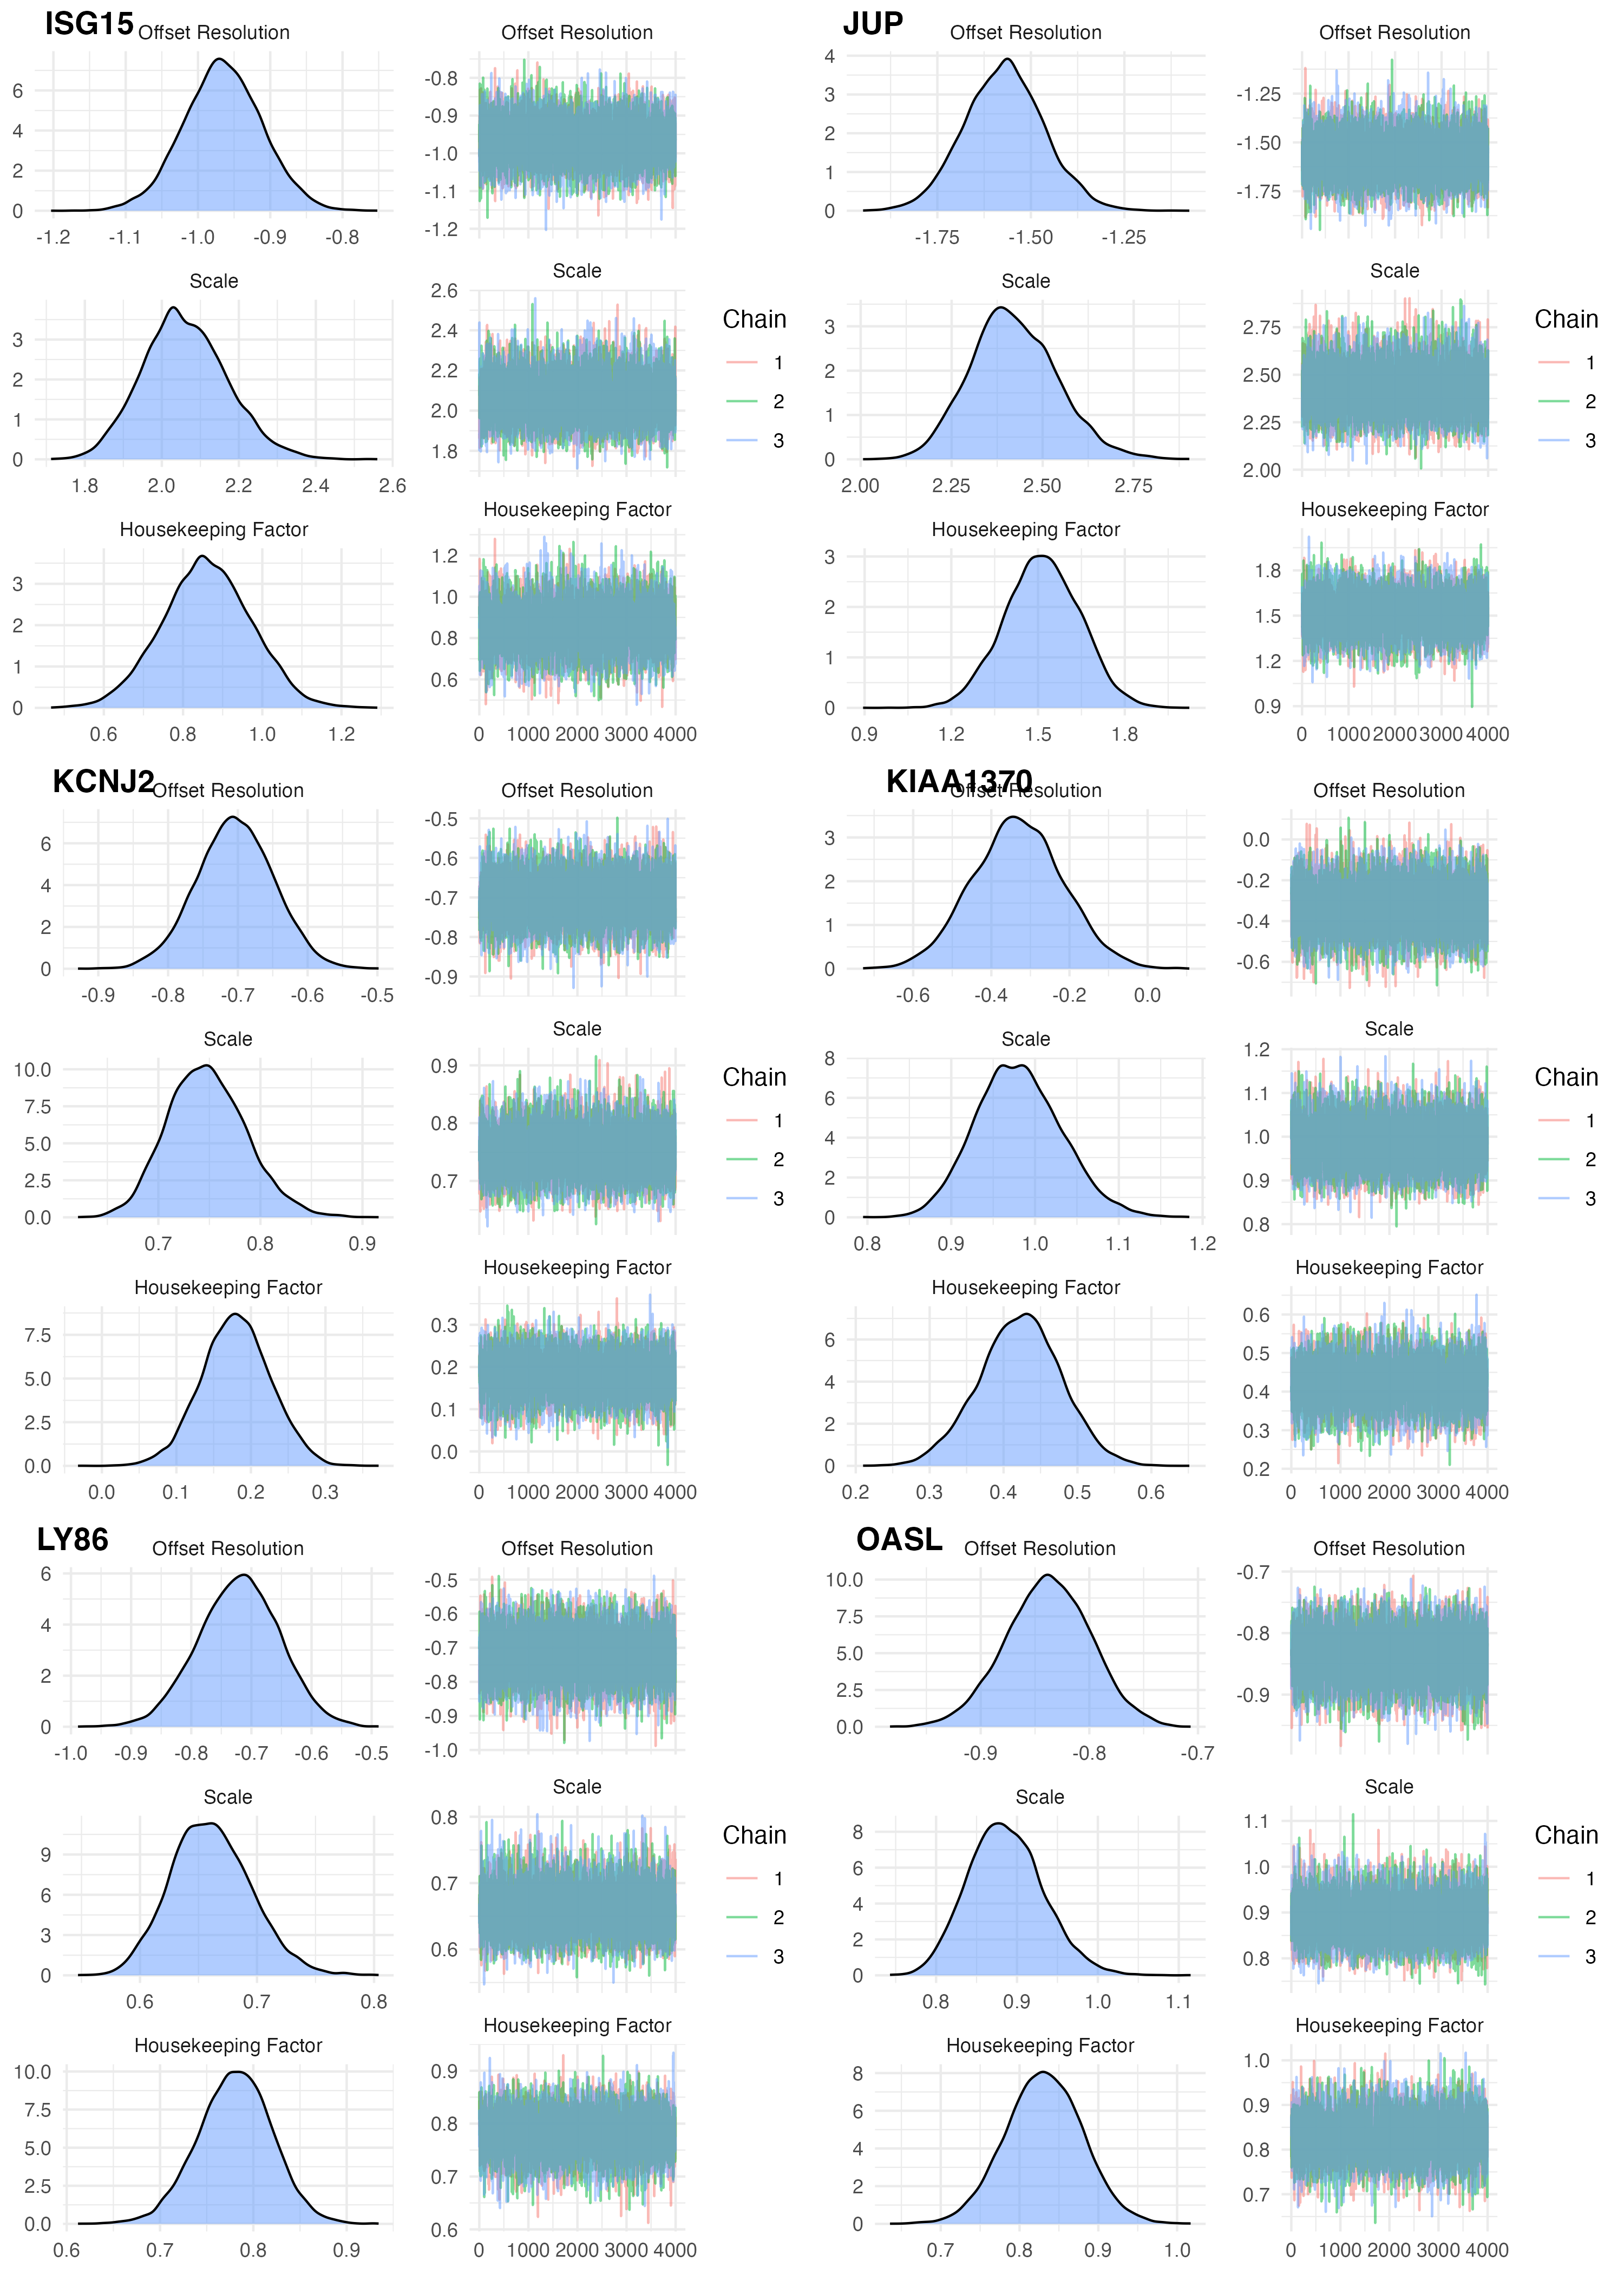
\includegraphics[width=\textwidth]{figures/chapter2/model_summaries_3.png}
    \caption{Model convergence summaries for each of the 25 single-target offset models summarised in Table~\ref{tab:single_target_offset_models_summary} (continued).}
    \label{fig:convergence_3}
\end{figure}

\begin{figure}
    \centering
    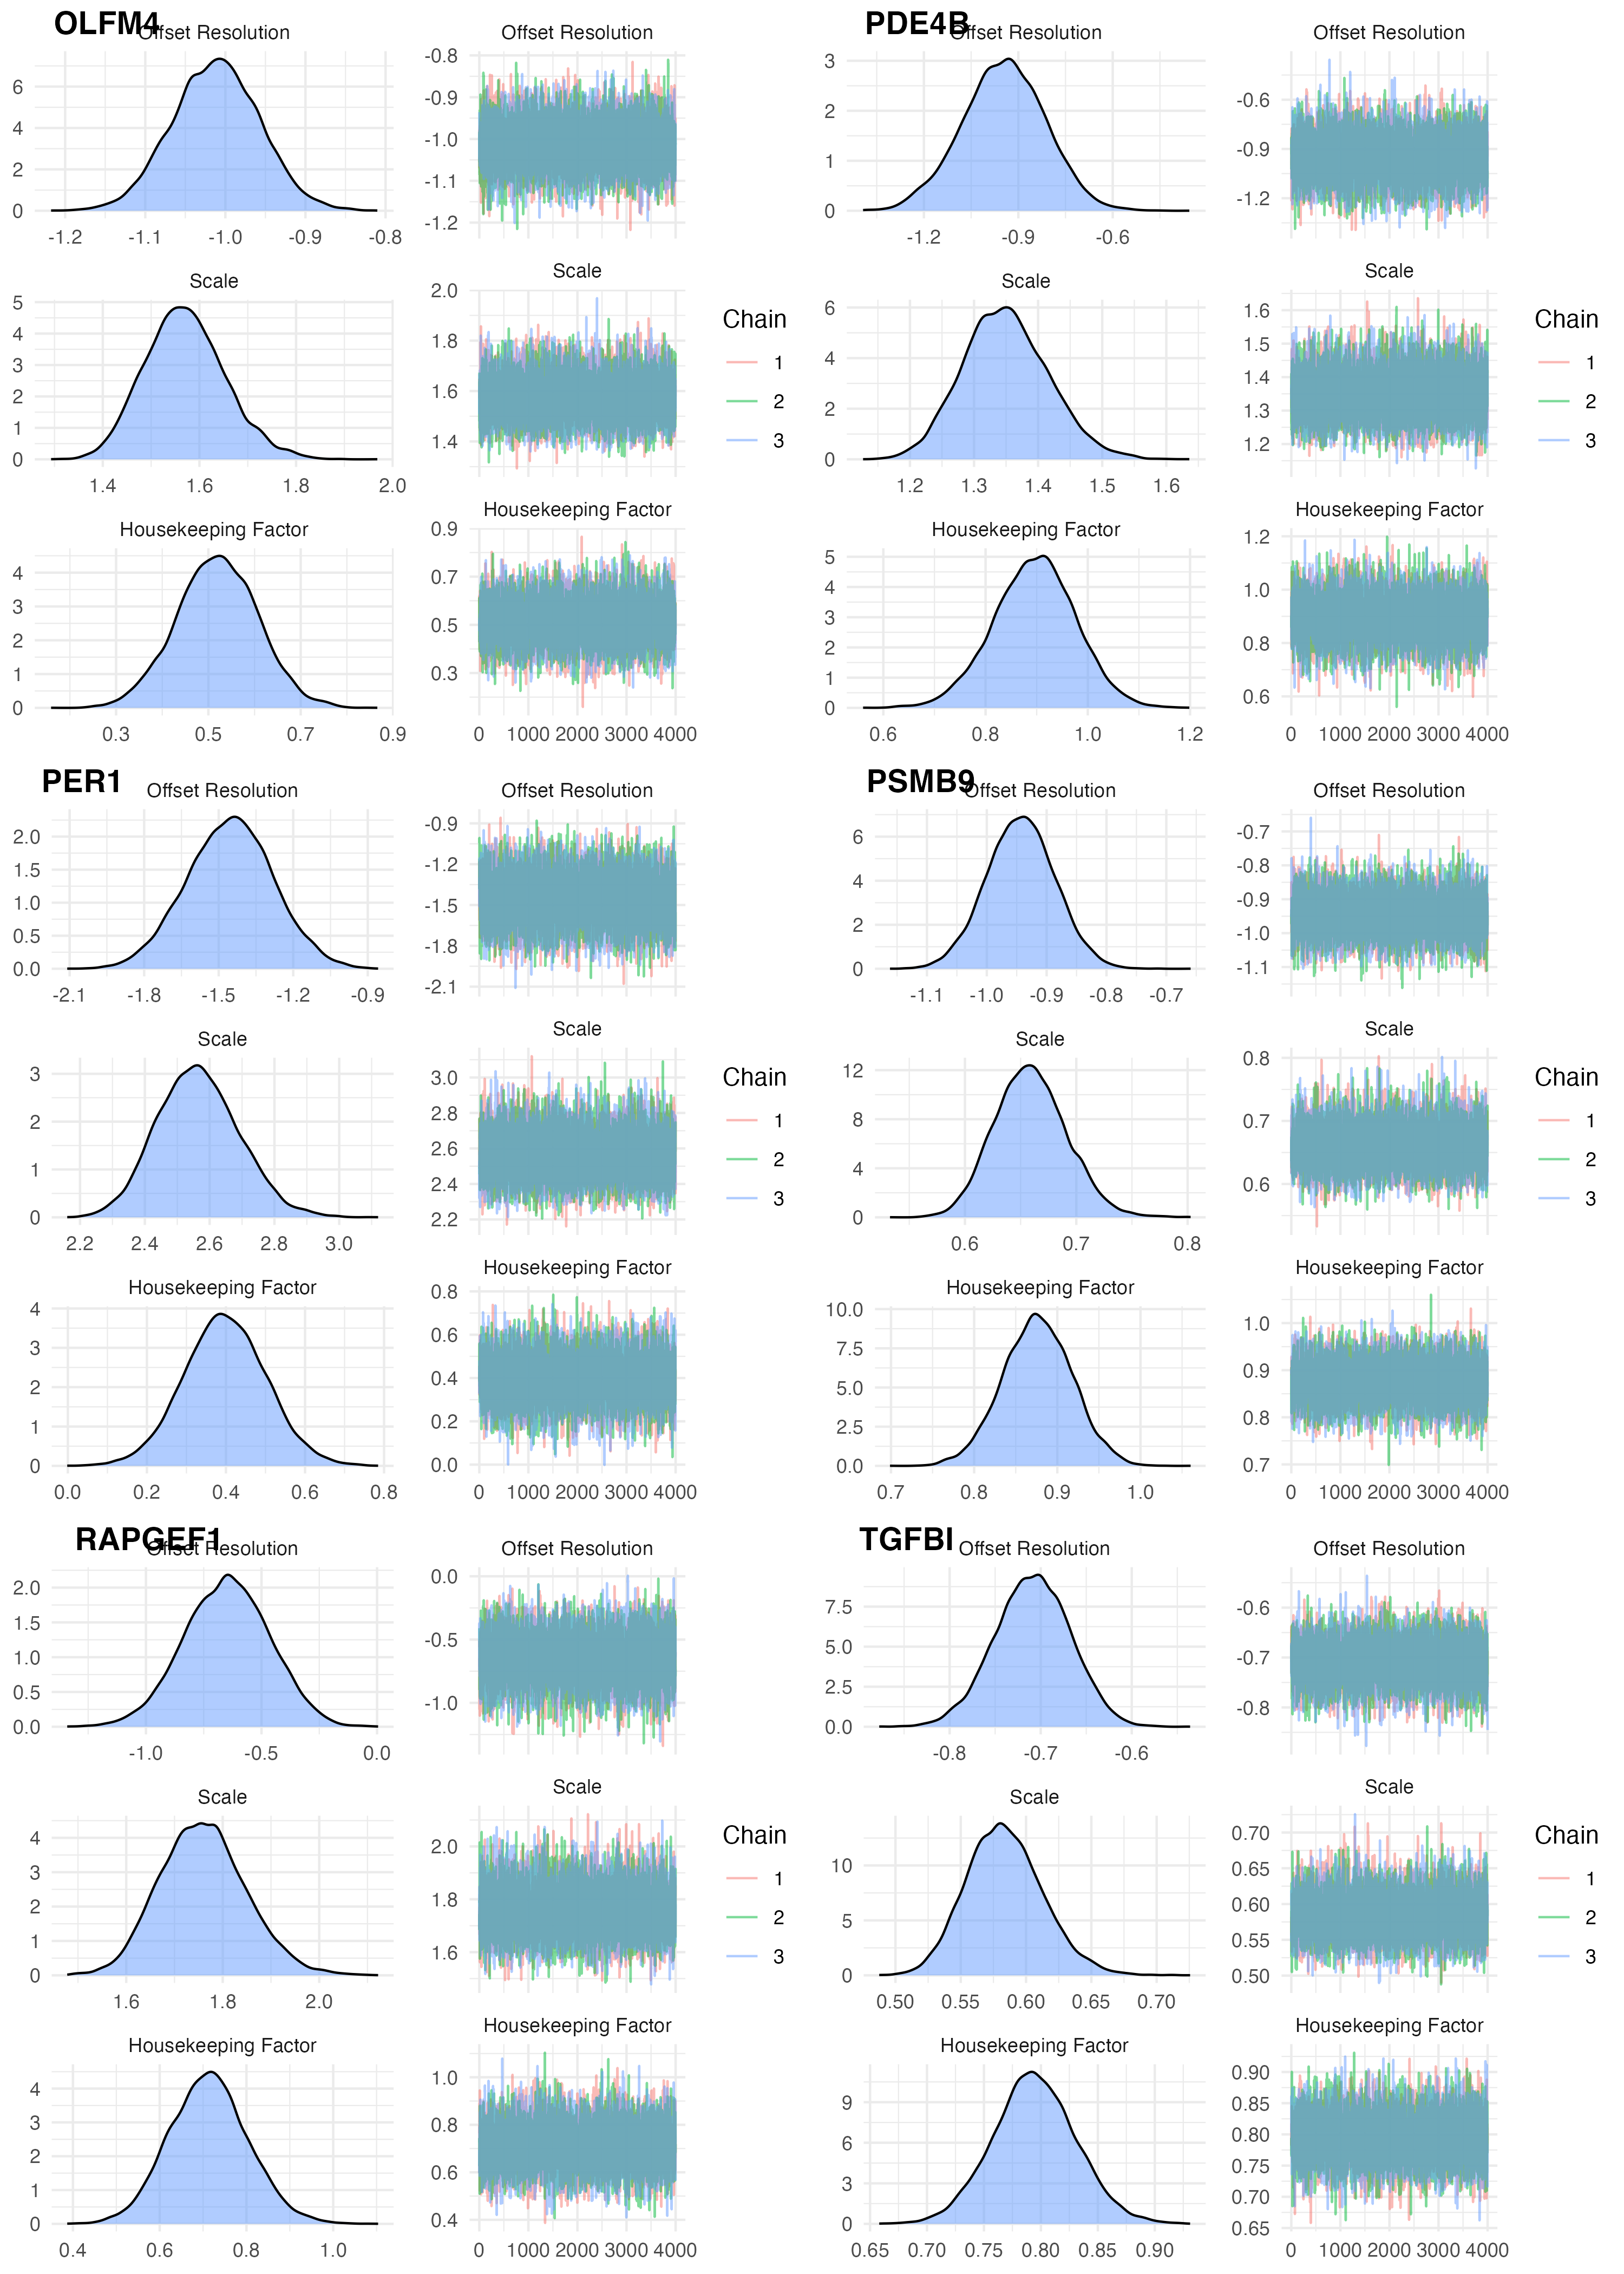
\includegraphics[width=\textwidth]{figures/chapter2/model_summaries_4.png}
    \caption{Model convergence summaries for each of the 25 single-target offset models summarised in Table~\ref{tab:single_target_offset_models_summary} (continued).}
    \label{fig:convergence_4}
\end{figure}

\dobib % renders bibliography (only when compiling for chapter only)
 
\end{document}